%\documentclass[11pt]{article}
%\usepackage[utf8]{inputenc}
%\usepackage[spanish]{babel}
%\usepackage[]{graphicx}
%\usepackage{colortbl} %para las tablas
%\usepackage{longtable} %para las tablas
%\usepackage{geometry}
%\geometry{tmargin=3cm,bmargin=3cm,lmargin=3cm,rmargin=2cm}
%
%\begin{document}

La siguiente es la estructura que se seguira para cada iteración:
\begin{enumerate}
        \item Análisis de Requerimientos del Sistema.
        \item Creación y Modificación de los diferentes Artefactos.
        \item Implementación.
\end{enumerate}
        \subsection{Descripción de subsistema}
        Para cada una de las iteraciones se debe tener en cuenta:
        \begin{enumerate}
                \item El mejoramiento de los requisitos planteados, ya sea su adicion, eliminación
                y/o modificación para que cumplan con los objetivos principales del sistema:
                Gestion de usuarios, Catalogación de Documentos, Consultas de usuarios y reportes.
                Esto se debe realizar para cada uno de los entregables establecidos en la sección
                de requerimientos. Es fundamental que cada uno de los integrantes del grupo de
                desarrolladores y los representantes del proyecto participen de dicho proceso.
             
                \item El mejoramiento de los artefactos y la adición de nuevos para cada uno de los
                entregables estipulados en las fechas de entrega. Se repartiran entre los
                diferentes integrantes la creación de los artefactos y en el mejoramiento de estos
                deberán participar todos los integrantes del equipo de desarrollo.
                
                \item La Implementación se realizará al finalizar el proceso de desarrollo en el
                último entregable con la particiación de los integrantes del grupo de 
                desarrolladores.
        \end{enumerate}
        
        %*********************************************************************       
        \subsection{Diagramas de caso de uso}
    		%\documentclass[11pt]{article}
%\usepackage[utf8]{inputenc}
%\usepackage[spanish]{babel}
%\usepackage[]{graphicx}
%\usepackage{colortbl} %para las tablas
%\usepackage{longtable} %para las tablas
%\usepackage{geometry}
%\geometry{tmargin=3cm,bmargin=3cm,lmargin=3cm,rmargin=2cm}

%\begin{document}
\begin{minipage}[c]{1\linewidth}
	\centering
    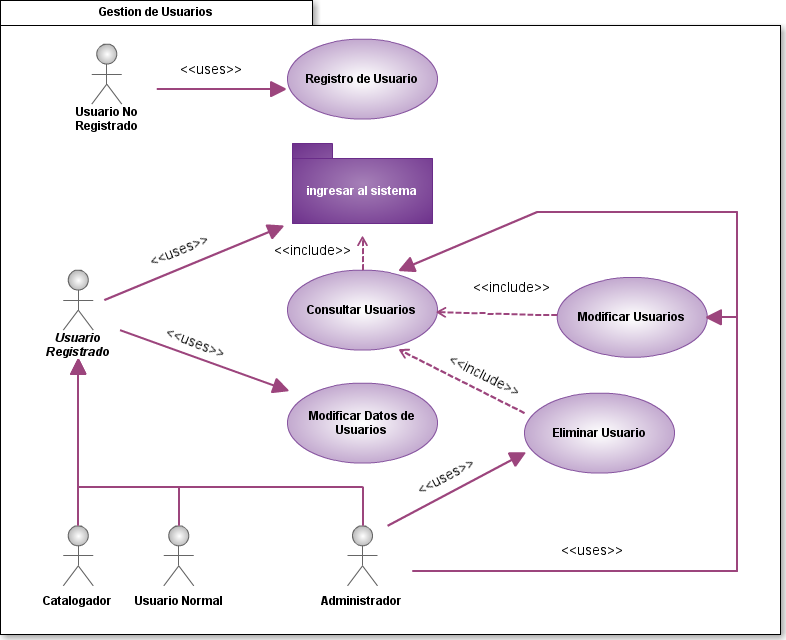
\includegraphics[scale=.6]{casosUso/CUGestionUsuarios}\\[0.5cm]
               
    \begin{tabular}{|p{0.225\textwidth}|p{0.225\textwidth}|p{0.225\textwidth}|p{0.225\textwidth}|}
    \hline
    {\bf Creador por} & {Edgar Andrés Moncada} & {\bf Fecha} & {Abril 03 2011}\\
    \hline
    \hline
    {\bf Actualizado}&{\bf Fecha}&\multicolumn{2}{p{0.45\textwidth}|}{\bf Observación}\\
    \hline
    {Edgar Andrés Moncada}&{Abril 4 2011}&\multicolumn{2}{p{0.45\textwidth}|}{Simplifico el
    diagrama quitando casos de uso innecesarios}\\
    \hline
    {Edgar Andrés Moncada}&{Abril 21 2011}&\multicolumn{2}{p{0.45\textwidth}|}{Adicionando la
    herencia del autor usuario registrado}\\
    \hline	
    {Cristian Ríos}&{Mayo 14 2011}&\multicolumn{2}{p{0.45\textwidth}|}{Se eliminó el caso de uso Eliminar Usuario}\\
    \hline	
    \end{tabular}
\end{minipage}     

%-------------------------------------------------------------------------------
  
\begin{minipage}[c]{1\linewidth}
	\centering
    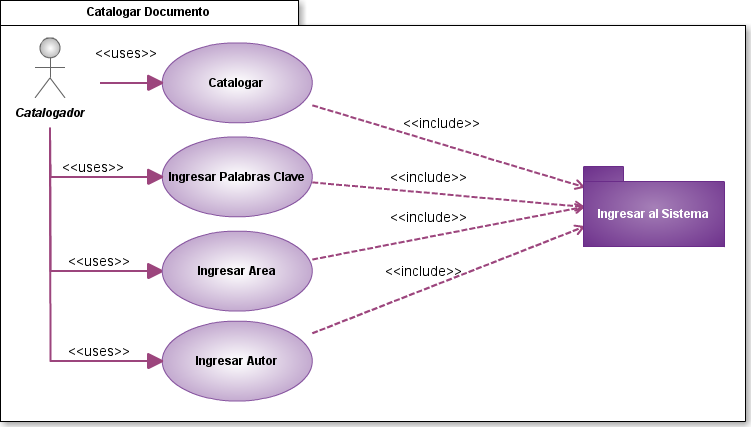
\includegraphics[width=16cm, height=14cm]{casosUso/CUCatalogar}\\[0.5cm]
                
    \begin{tabular}{|p{0.225\textwidth}|p{0.225\textwidth}|p{0.225\textwidth}|p{0.225\textwidth}|}
    \hline
    {\bf Autor} & {Luis Felipe Vargas} & {\bf Fecha} & {Abril 05 2011}\\
    \hline
    \hline
    {\bf Actualizado por}& {\bf Fecha} & \multicolumn{2}{p{0.45\textwidth}|} {\bf Observación}\\
    \hline
    {Cristian Ríos}&{Mayo 14 2011}&\multicolumn{2}{p{0.45\textwidth}|}{Se agrego el caso de uso Ingresar Tipo Material}\\
    \hline	
    \end{tabular}
\end{minipage}\\[5cm]

%-------------------------------------------------------------------------------
       
\begin{minipage}[c]{1\linewidth}
	\centering
    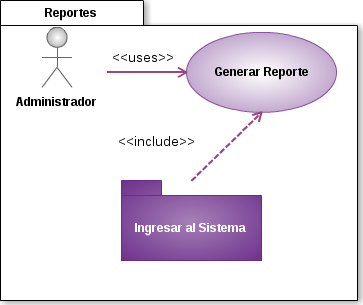
\includegraphics[scale=.7]{casosUso/CUReportes}\\[0.5cm]
                
    \begin{tabular}{|p{0.225\textwidth}|p{0.225\textwidth}|p{0.225\textwidth}|p{0.225\textwidth}|}
    \hline
    {\bf Autor} & {Edgar Andrés Moncada} & {\bf Fecha} & {Abril 03 2011}\\
    \hline
    \hline
    {\bf Actualizado por}& {\bf Fecha} & \multicolumn{2}{p{0.45\textwidth}|} {\bf Observación}\\
    \hline
    {Edgar Andrés Moncada}& {Abril 29 2011} & \multicolumn{2}{p{0.45\textwidth}|} {Se quitaron los
    casos de uso que extendían y se dejo un solo caso de generar reporte}\\
    \hline
    {Edgar Andrés Moncada}& {Mayo 04 2011} & \multicolumn{2}{p{0.45\textwidth}|} {Se agrego el
     paquete ingresar al sistema}\\
    \hline
    \end{tabular}
\end{minipage}\\[1cm]

%-------------------------------------------------------------------------------
        
\begin{minipage}[c]{1\linewidth}
	\centering
	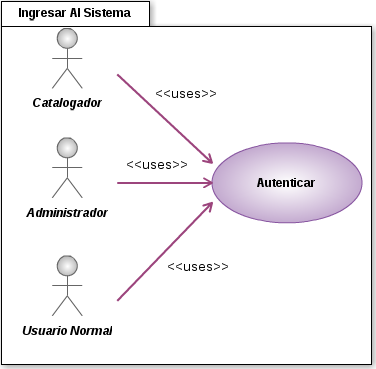
\includegraphics[scale=.6]{casosUso/CUAutenticar}\\[0.5cm]
               
    \begin{tabular}{|p{0.225\textwidth}|p{0.225\textwidth}|p{0.225\textwidth}|p{0.225\textwidth}|}
    \hline
    {\bf Autor} & {Edgar Andrés Moncada} & {\bf Fecha} & {Abril 04 2011}\\
    \hline
    %\hline
    %{\bf Actualizado por}& {\bf Fecha} & \multicolumn{2}{p{0.45\textwidth}|} {\bf Observación}\\
    %\hline	
    \end{tabular}                
\end{minipage}

%-------------------------------------------------------------------------------
       
\begin{minipage}[c]{1\linewidth}
	\centering
    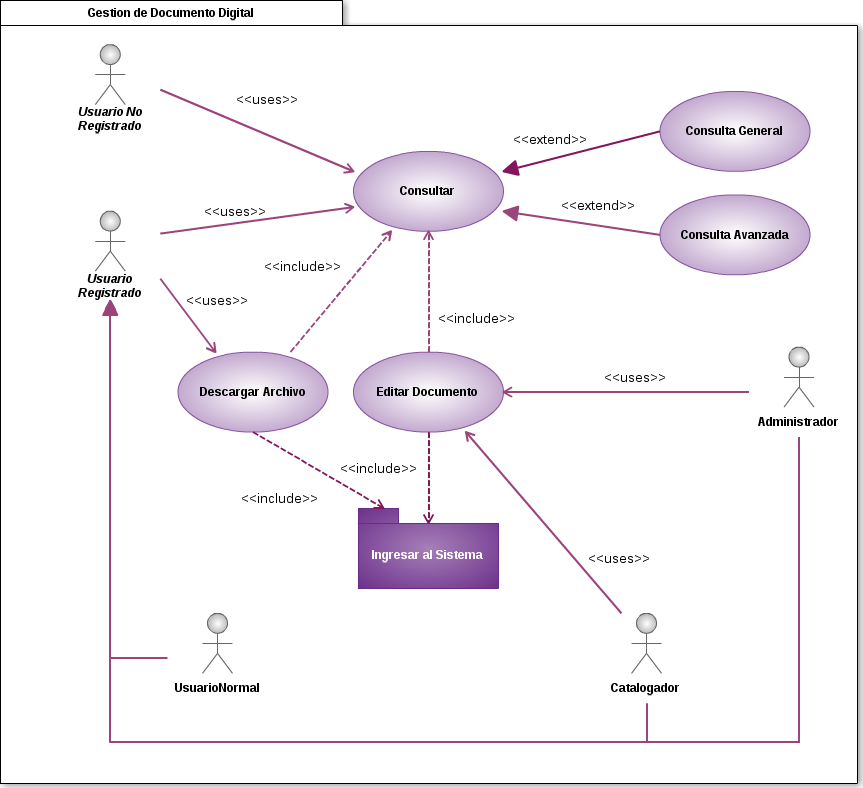
\includegraphics[scale=.5]{casosUso/CUGestionDocumento}\\[0.5cm]
               
    \begin{tabular}{|p{0.225\textwidth}|p{0.225\textwidth}|p{0.225\textwidth}|p{0.225\textwidth}|}
    \hline
    {\bf Creador por} & {Edgar Andrés Moncada} & {\bf Fecha} & {Abril 03 2011}\\
    \hline
    \hline
    {\bf Actualizado por}& {\bf Fecha} & \multicolumn{2}{p{0.45\textwidth}|} {\bf Observación}\\
    \hline
    {Edgar Andrés Moncada}& {Abril 04 2011} & \multicolumn{2}{p{0.45\textwidth}|} {Simplifico el
    diagrama quitando casos de uso innecesarios}\\
    \hline
    {Edgar Andrés Moncada}& {Abril 28 2011} & \multicolumn{2}{p{0.45\textwidth}|} {Se adiciona la
    herencia del actor UsuarioRegistrado}\\
    \hline
    {Edgar Andrés Moncada}& {Mayo 03 2011} & \multicolumn{2}{p{0.45\textwidth}|} {Se quita el caso
    de uso eliminar documento}\\
    \hline		
    \end{tabular}
\end{minipage}
 
%\end{document}    
	      
        
        \newpage                
             \subsubsection{Especificación de casos de uso}
                %\documentclass[]{article}
%\usepackage[spanish]{babel}
%\usepackage[utf8]{inputenc}
%\usepackage{geometry}
%\usepackage{colortbl}
%\usepackage{longtable}
%\usepackage{graphicx}
%\geometry{tmargin=3cm,bmargin=3cm,lmargin=3cm,rmargin=2cm}
%\begin{document}
\begin{center}
\begin{longtable}{|p{0.225\textwidth}|p{0.225\textwidth}|p{0.225\textwidth}|p{0.225\textwidth}|}
\hline
{\bf {Empresa:}} &
\multicolumn{2}{p{0.45\textwidth}|} { Escuela de Ingeniería de Sistemas y Computación } &
{
\includegraphics[width=80.5pt]{LOGO}} \\
\hline
\bf {Nombre del caso de uso:}&\multicolumn{3}{l|}{
Registro de Usuario.
} \\
\hline
\bf Código: & 
CU00 &\bf Fecha: & 
Abril 03 2011 \\
\hline
\bf Autor(es ): & 
Edgar Andrés Moncada & 
Yerminson Gonzalez & 
 \\
\hline
\bf Descripción: &\multicolumn{3}{p{0.675\textwidth}|}
{
Permite el registro al sistema de nuevos usuarios.
} \\
\hline
\bf Actores: &\multicolumn{3}{p{0.675\textwidth}|}{
Usuario No Registrado. 
} \\
\hline
\bf Precondiciones: &\multicolumn{3}{p{0.675\textwidth}|}
{
El sistema debe de haberse iniciado.
} \\
\hline
\multicolumn{4}{|c|}{\bf {Flujo Normal}}\\
\hline
\multicolumn{2}{|c}{\bf Actor} & \multicolumn{2}{|c|}{\bf Sistema } \\
\hline
\multicolumn{2}{|p{0.45\textwidth}}
{
\begin{itemize}
\item [1.]El caso de uso inicia cuando el usuario no registrado selecciona la opción de registrarse.
\item [3.] El usuario digita los campos pedidos.
\item[4.] El usuario le indica al sistema que valide los datos.
\end{itemize}
} &
\multicolumn{2}{|p{0.45\textwidth}|}
{
\begin{itemize}
\item[2.] El sistema genera una interfaz que le pide al usuario los siguientes datos obligatorios: login, contraseña, verificación de la contraseña, pregunta y respuesta secreta, nombre. A demás pide los siguientes datos que no son obligatorios: apellidos, género, fecha de nacimiento, email, nivel de escolaridad, vinculo con Univalle (estudiante de pregrado, de posgrado, egresado, profesor activo, jubilado, ninguno). Se pide información sobre las aéreas de interés.
\item[5.] El Sistema valida que el login no exista.
\item[6.] El Sistema valida que los campos de contraseña y verificación de contraseña.
 El sistema valida los campos digitados.
\item[7.] El sistema crea una nueva instancia del usuario en la base de datos.
\item[8.] El sistema envía un mensaje de confirmación al usuario y el caso de uso termina.
\end{itemize}
} \\
\hline
\multicolumn{4}{|c|}{\bf {Flujo Alternativo}}\\
\hline
\multicolumn{2}{|p{0.45\textwidth}}
{
\begin{itemize}
\item[3.3.] El Usuario no digita ninguno de los campos obligatorios.
\item[4.3.] El Usuario le indica al Sistema que valide los datos.
\end{itemize}
} &
\multicolumn{2}{|p{0.45\textwidth}|}
{
\begin{itemize}
\item[5.1.] El Sistema al validar se da cuenta que el login digitado por el Usuario ya existe.
\item[6.1. ]El Sistema envía una notificación al usuario indicándole que ingrese un nuevo login.
\item[6.2. ]El Sistema al validar se da cuenta que el campo de contraseña y el campo de verificación de contraseña no son iguales.
\item[7.2. ]El Sistema envía una notificación al Usuario indicándole que las contraseñas no coinciden y que las vuelva a confirmar.
\item[5.3. ]El Sistema al validar se da cuenta que los campos obligatorios no tienen datos.
\item[6.3.] El Sistema envía una notificación al Usuario indicándole que vuelva a confirmar.
\end{itemize}
} \\
\hline
\bf Poscondiciones: &\multicolumn{3}{p{0.675\textwidth}|}
{
El sistema almacena los datos del usuario en la base de datos.
} \\
\hline
\bf Excepciones: &\multicolumn{3}{p{0.675\textwidth}|}
{
El sistema no puede acceder a la base de datos y no puede almacenar los datos.
} \\
\hline
\bf Aprobado por : & 
 & \bf Fecha & 
 \\
\hline
\end{longtable}
\end{center}
%\end{document}
                %%\pagebreak
                        
                %\documentclass[]{article}
%\usepackage[spanish]{babel}
%\usepackage[utf8]{inputenc}
%\usepackage{geometry}
%\usepackage{colortbl}
%\usepackage{longtable}
%\usepackage{graphicx}
%\geometry{tmargin=3cm,bmargin=3cm,lmargin=3cm,rmargin=2cm}
%
%\begin{document}

\begin{center}
\begin{longtable}{|p{0.225\textwidth}|p{0.225\textwidth}|p{0.225\textwidth}|p{0.225\textwidth}|}
\hline
{\bf {Empresa:}} &
\multicolumn{2}{p{0.45\textwidth}|} { Escuela de Ingeniería de Sistemas y Computación } &
{
\includegraphics[width=80.5pt]{LOGO}} \\
\hline
\bf {Nombre del caso de uso:}&\multicolumn{3}{l|}{
Autenticar.
} \\
\hline
\bf Codigo: & 
CU01 &\bf Fecha: & 
Abril 02 2011 \\
\hline
\bf Autor(es ): & 
Edgar Andrés Moncada & 
 & 
 \\
\hline
\bf Descripcion: &\multicolumn{3}{p{0.675\textwidth}|}
{
Permite el ingreso y autenticación de los usuarios al sistema.
} \\
\hline
\bf Actores: &\multicolumn{3}{p{0.675\textwidth}|}{
Administrador, Catalogador, Usuario Normal. 
} \\
\hline
\bf Precondiciones: &\multicolumn{3}{p{0.675\textwidth}|}
{
Estar registrado en la biblioteca.
} \\
\hline
\multicolumn{4}{|c|}{\bf {Flujo Normal}}\\
\hline
\multicolumn{2}{|c}{\bf Actor} & \multicolumn{2}{|c|}{\bf Sistema } \\
\hline
\multicolumn{2}{|p{0.45\textwidth}}
{
\begin{itemize}
\item[1.] El Usuario selecciona la opción ingresar a la biblioteca.
\item[3.] El Usuario rellena los respectivos campos con su login y su contraseña y selecciona la opción ingresar.
\end{itemize}
} &
\multicolumn{2}{|p{0.45\textwidth}|}
{
\begin{itemize}
\item[2.] El sistema muestra los campos de login y contraseña.
\item[4.] El sistema verifica que el login exista y que la contraseña corresponde con la que se tiene almacenada.
\item[5.] El sistema actualiza el estado del usuario y el caso de uso termina.
\end{itemize}
} \\
\hline
\multicolumn{4}{|c|}{\bf {Flujo Alternativo}}\\
\hline
\multicolumn{2}{|p{0.45\textwidth}}
{} &
\multicolumn{2}{|p{0.45\textwidth}|}
{
\begin{itemize}
\item[4.1.]El Sistema alverificar se da cuenta que el login digitado por el usuario no existe
\item[5.1.]El Sistema indica que no existe el login y pide al usuario los datos de nuevo.
\item[4.2.] El Sistema al verificar se da cuenta que la contraseña digitada por el Usuario es errónea.
\item[5.2.] El Sistema envía una notificación indicando que la contraseña es errónea y que repita el proceso.
\end{itemize}
} \\
\hline
\bf Poscondiciones: &\multicolumn{3}{p{0.675\textwidth}|}
{
El sistema actualiza el perfil de usuario. El usuario identificado esta activo en el sistema.
} \\
\hline
\bf Excepciones: &\multicolumn{3}{p{0.675\textwidth}|}
{
El sistema no puede acceder a la base de datos y no puede verificar el login y/o la contraseña del usuario.
} \\
\hline
\bf Aprobado por : & 
 & \bf Fecha & 
 \\
\hline
\end{longtable}
\end{center}
%\end{document}
                 %%\pagebreak
                        
                 %\documentclass[]{article}
%\usepackage[spanish]{babel}
%\usepackage[utf8]{inputenc}
%\usepackage{geometry}
%\usepackage{colortbl}
%\usepackage{longtable}
%\usepackage{graphicx}
%\geometry{tmargin=3cm,bmargin=3cm,lmargin=3cm,rmargin=2cm}
%
%\begin{document}
\begin{center}
\begin{longtable}{|p{0.225\textwidth}|p{0.225\textwidth}|p{0.225\textwidth}|p{0.225\textwidth}|}
\hline
{\bf {Empresa:}} &
\multicolumn{2}{p{0.45\textwidth}|} { Escuela de Ingeniería de Sistemas y Computación } &
{
\includegraphics[width=80.5pt]{LOGO}} \\
\hline
\bf {Nombre del caso de uso:}&\multicolumn{3}{l|}{
Modificar usuarios.
} \\
\hline
\bf Codigo: & 
CU02 &\bf Fecha: & 
Abril 2 2011 \\
\hline
\bf Autor(es ): & 
Yerminson Gonzalez & 
Edgar Andrés Moncada & 
 \\
\hline
\bf Descripcion: &\multicolumn{3}{p{0.675\textwidth}|}
{
Permite la modificación de usuarios , es decir alguna de la información almacenada en el sistema.
} \\
\hline
\bf Actores: &\multicolumn{3}{p{0.675\textwidth}|}{
Administrador. 
} \\
\hline
\bf Precondiciones: &\multicolumn{3}{p{0.675\textwidth}|}
{
El administrador debe haber consultado sobre algún usuario.
} \\
\hline
\multicolumn{4}{|c|}{\bf {Flujo Normal}}\\
\hline
\multicolumn{2}{|c}{\bf Actor} & \multicolumn{2}{|c|}{\bf Sistema } \\
\hline
\multicolumn{2}{|p{0.45\textwidth}}
{
\begin{itemize}
\item[1. ]El caso de uso inicia cuando el administrador selecciona al usuario de la lista resultado.
\item[3.] El administrador modifica los datos de acuerdo a sus necesidades o ha una actualización de datos.
\end{itemize}
} &
\multicolumn{2}{|p{0.45\textwidth}|}
{
\begin{itemize}
\item[2.] El sistema responde a través de una interfaz que muestra los campos referente a sus atributos, donde se pueden modificar el estado o el perfil de algún usuario seleccionado el dato perfil de usuario puede ser: Usuario normal, Catalogador o administrador, el dato estado puede ser: Habilitado o deshabilitado.
\item[4. ]El sistema valida que todos los datos obligatorios se hayan suministrado.
\item[5. ]El sistema accede a la base de datos y realiza una verificación de los datos nuevos y existentes para que no hayan datos iguales donde no pueden serlo.
\item[6.] El sistema realiza la actualización de los datos en la base de datos con los datos suministrados según la preferencia del administrador.
\item[7.] El sistema responde a través de una interfaz de éxito donde muestra que se ha completado la operación y el caso de uso termina.
\end{itemize}
} \\
\hline
\multicolumn{4}{|c|}{\bf {Flujo Alternativo}}\\
\hline
\multicolumn{2}{|p{0.45\textwidth}}
{} &
\multicolumn{2}{|p{0.45\textwidth}|}
{
\begin{itemize}
\item[4.1.] El Sistema valida los datos y encuentra que hay errores.
\item[4.2.] El Sistema responde a través de una interfaz que muestra los campos referentes a los atributos para que sean llenados nuevamente, con información del error cometido.
\end{itemize}
} \\
\hline
\bf Poscondiciones: &\multicolumn{3}{p{0.675\textwidth}|}
{
Atributos de usuario en la base de datos modificados.
} \\
\hline
\bf Excepciones: &\multicolumn{3}{p{0.675\textwidth}|}
{
La base de datos puede desconectarse debido a fallos de energía.
} \\
\hline
\bf Aprobado por : & 
 & \bf Fecha & 
 \\
\hline
\end{longtable}
\end{center}
%\end{document}
                 %%\pagebreak
                        
                  %\documentclass[]{article}
%\usepackage[spanish]{babel}
%\usepackage[utf8]{inputenc}
%\usepackage{geometry}
%\usepackage{colortbl}
%\usepackage{longtable}
%\usepackage{graphicx}
%\geometry{tmargin=3cm,bmargin=3cm,lmargin=3cm,rmargin=2cm}
%
%\begin{document}
\begin{center}
\begin{longtable}{|p{0.225\textwidth}|p{0.225\textwidth}|p{0.225\textwidth}|p{0.225\textwidth}|}
\hline
{\bf {Empresa:}} &
\multicolumn{2}{p{0.45\textwidth}|} { Escuela de Ingeniería de Sistemas y Computación } &
{
\includegraphics[width=80.5pt]{LOGO}} \\
\hline
\bf {Nombre del caso de uso:}&\multicolumn{3}{l|}{
Modificar datos usuario.
} \\
\hline
\bf Codigo: & 
CU03 &\bf Fecha: & 
Abril 02 2011 \\
\hline
\bf Autor(es ): & 
Edgar Andrés Moncada & 
Yerminson Gonzalez & 
 \\
\hline
\bf Descripcion: &\multicolumn{3}{p{0.675\textwidth}|}
{
Permite la modificación de algunos datos del usuario.
} \\
\hline
\bf Actores: &\multicolumn{3}{p{0.675\textwidth}|}{
Usuario norma, Catalogador	y Administrador. 
} \\
\hline
\bf Precondiciones: &\multicolumn{3}{p{0.675\textwidth}|}
{
El usuario debe haberse logueado en el sistema.
} \\
\hline
\multicolumn{4}{|c|}{\bf {Flujo Normal}}\\
\hline
\multicolumn{2}{|c}{\bf Actor} & \multicolumn{2}{|c|}{\bf Sistema } \\
\hline
\multicolumn{2}{|p{0.45\textwidth}}
{
\begin{itemize}
\item[1. ]El caso de uso inicia cuando el usuario solicita editar su perfil.
\item[3. ]El usuario modifica los datos correspondientes de acuerdo a sus necesidades o ha una actualización de datos.
\end{itemize}
} &
\multicolumn{2}{|p{0.45\textwidth}|}
{
\begin{itemize}
\item[2. ]El sistema responde a través de una interfaz que muestra los campos referente a sus atributos, con los siguientes datos editables: contraseña, pregunta y respuesta secreta, nombre, apellidos, género, fecha nacimiento, nivel escolaridad, vinculo con univalle y áreas de interés. Los demás campos no son editables.
\item[4. ]El sistema valida de que los campos obligatorios contengan datos.
\item[5. ]El sistema accede a la base de datos y valida que los datos existentes y los nuevos datos no sean iguales cuando no pueden serlo.
\item[6. ]El sistema accede a la base de datos, y actualiza los valores de acuerdo a los suministrados por el usuario.
\item[7. ]El sistema responde a través de una interfaz de éxito donde muestra que se ha completado la operación.
 \end{itemize}
} \\
\hline
\multicolumn{4}{|c|}{\bf {Flujo Alternativo}}\\
\hline
\multicolumn{2}{|p{0.45\textwidth}}
{} &
\multicolumn{2}{|p{0.45\textwidth}|}
{
\begin{itemize}
\item[5.1.] El Sistema al validar los datos encuentra un error debido a que  el usuario lleno de manera incorrecta alguno de los campos correspondiente a la información editable  como: contraseña, pregunta y respuesta secreta, nombre, apellidos, género, fecha nacimiento, nivel escolaridad, vinculo con Univalle y áreas de interés.
\item[6.1.] El Sistema responde a través de una interfaz que muestra los campos referentes a los atributos para que sean llenados nuevamente, con información del error cometido.
\end{itemize} 
} \\
\hline
\bf Poscondiciones: &\multicolumn{3}{p{0.675\textwidth}|}
{
Atributos de usuario en la base de datos modificados.
} \\
\hline
\bf Excepciones: &\multicolumn{3}{p{0.675\textwidth}|}
{
La base de datos puede desconectarse debido a fallos de energía.
} \\
\hline
\bf Aprobado por : & 
 & \bf Fecha & 
 \\
\hline
\end{longtable}
\end{center}
%\end{document}
                  %%\pagebreak        
                       
                  %\documentclass[]{article}
%\usepackage[spanish]{babel}
%\usepackage[utf8]{inputenc}
%\usepackage{geometry}
%\usepackage{colortbl}
%\usepackage{longtable}
%\usepackage{graphicx}
%\geometry{tmargin=3cm,bmargin=3cm,lmargin=3cm,rmargin=2cm}
%
%\begin{document}
\begin{center}
\begin{longtable}{|p{0.225\textwidth}|p{0.225\textwidth}|p{0.225\textwidth}|p{0.225\textwidth}|}
\hline
{\bf {Empresa:}} &
\multicolumn{2}{p{0.45\textwidth}|} { Escuela de Ingeniería de Sistemas y Computación } &
{
\includegraphics[width=80.5pt]{LOGO}} \\
\hline
\bf {Nombre del caso de uso:}&\multicolumn{3}{l|}{
Ingresar tipos de material.
} \\
\hline
\bf Código: & 
CU07 &\bf Fecha: & 
Mayo 04 2011 \\
\hline
\bf Autor(es ): & 
Yerminson Gonzalez & 
 & 
 \\
\hline
\bf Descripción: &\multicolumn{3}{p{0.675\textwidth}|}
{
Permite la creación de nuevos tipos de material en caso de que se requiera para registro de un documento y que den información sobre la estructura del documento.
} \\
\hline
\bf Actores: &\multicolumn{3}{p{0.675\textwidth}|}{
Administrador y Catalogador. 
} \\
\hline
\bf Precondiciones: &\multicolumn{3}{p{0.675\textwidth}|}
{
Haber ingresado al sistema y tener perfil de catalogador o administrador.
} \\
\hline
\multicolumn{4}{|c|}{\bf {Flujo Normal}}\\
\hline
\multicolumn{2}{|c}{\bf Actor} & \multicolumn{2}{|c|}{\bf Sistema } \\
\hline
\multicolumn{2}{|p{0.45\textwidth}}
{
\begin{itemize}
\item[1. ]El caso de uso inicia cuando el catalogador solicita crear un tipo de material para algún documento.
\item[3.] El usuario ingresa datos en los campos proporcionado por la interfaz del sistema para creación de nuevos tipos de material.
\item[4. ]El usuario indica al sistema que ya a ingresado los datos y que desea crear el nuevo tipo de material.
\item[7. ]El usuario acepta el mensaje de confirmación generado por el sistema y el caso de uso finaliza.
\end{itemize}
} &
\multicolumn{2}{|p{0.45\textwidth}|}
{
\begin{itemize}
\item[2.] El sistema responde mostrando una interfaz con dos campos: un campo para indicar el nombre y un campo para indicar una descripción del tipo.
\item[5.] El sistema valida que el nombre del tipo de material que ha ingresado el usuario para el nuevo tipo de material no exista como nombre de otro tipo de material.
\item[6. ]El sistema crea un nuevo tipo de material para documentos de ciencias de la computación que serán almacenados en el sistema y responde con un mensaje al usuario indicando el éxito de la operación.
\end{itemize}
} \\
\hline
\multicolumn{4}{|c|}{\bf {Flujo Alternativo}}\\
\hline
\multicolumn{2}{|p{0.45\textwidth}}
{
\begin{itemize}
\item[7.1] El usuario acepta el mensaje de notificación del error generado por el sistema.
\end{itemize}
} &
\multicolumn{2}{|p{0.45\textwidth}|}
{
\begin{itemize}
\item[5.1] El sistema al realizar la validación del nombre se percata de que el nombre dado al nuevo tipo de material ya existe.
\item[6.1] El sistema genera un mensaje indicando que el nombre dado al tipo de material no se puede utilizar porque ya existe un tipo de material con ese nombre.
\end{itemize}
} \\
\hline
\bf Poscondiciones: &\multicolumn{3}{p{0.675\textwidth}|}
{
El sistema añade un registro correspondiente a los tipos de material a los que pueden pertenecer los documentos.
} \\
\hline
\bf Excepciones: &\multicolumn{3}{p{0.675\textwidth}|}
{
Fallo de conexionen la base de datos.	Falla en el sistema de suministro de energía.
} \\
\hline
\bf Aprobado por : & 
 & \bf Fecha & 
 \\
\hline
\end{longtable}
\end{center}
%\end{document}
                  %\pagebreak                                
                        
                  %\documentclass[]{article}
%\usepackage[spanish]{babel}
%\usepackage[utf8]{inputenc}
%\usepackage{geometry}
%\usepackage{colortbl}
%\usepackage{longtable}
%\usepackage{graphicx}
%\geometry{tmargin=3cm,bmargin=3cm,lmargin=3cm,rmargin=2cm}
%
%\begin{document}
\begin{center}
\begin{longtable}{|p{0.225\textwidth}|p{0.225\textwidth}|p{0.225\textwidth}|p{0.225\textwidth}|}
\hline
{\bf {Empresa:}} &
\multicolumn{2}{p{0.45\textwidth}|} { Escuela de Ingeniería de Sistemas y Computación } &
{
\includegraphics[width=80.5pt]{LOGO}} \\
\hline
\bf {Nombre del caso de uso:}&\multicolumn{3}{l|}{
Consultar usuarios.
} \\
\hline
\bf Código: & 
CU05 &\bf Fecha: & 
Abril 02 2011 \\
\hline
\bf Autor(es ): & 
Edgar Andrés Moncada & 
Yerminson Gonzalez & 
 \\
\hline
\bf Descripción: &\multicolumn{3}{p{0.675\textwidth}|}
{
Permite la consulta de usuarios que están registrados al sistema.
} \\
\hline
\bf Actores: &\multicolumn{3}{p{0.675\textwidth}|}{
Administrador. 
} \\
\hline
\bf Precondiciones: &\multicolumn{3}{p{0.675\textwidth}|}
{
El usuario debe haberse autentificado en el sistema y tener perfil de administrador.
} \\
\hline
\multicolumn{4}{|c|}{\bf {Flujo Normal}}\\
\hline
\multicolumn{2}{|c}{\bf Actor} & \multicolumn{2}{|c|}{\bf Sistema } \\
\hline
\multicolumn{2}{|p{0.45\textwidth}}
{
\begin{itemize}
\item[1. ]El caso de uso inicia cuando el cliente solicita la consulta de usuarios.
\item[3. ]El administrador escribe las palabras claves con respecto a la búsqueda y solicita al sistema que se realiza la búsqueda.
\end{itemize}
} &
\multicolumn{2}{|p{0.45\textwidth}|}
{
\begin{itemize}
 \item[2.] El sistema responde a través de una interfaz que permite introducir las palabras claves por las cuales se desea buscar algún usuario.
\item[4.] El sistema envía la consulta a la base de datos y con la información obtenida genera una interfaz donde muestra de manera organiza los resultados obtenidos.
\item[5.] El sistema envía esta interfaz al usuario como resultado de su consulta y el caso de uso termina.
\end{itemize}
} \\
\hline
\multicolumn{4}{|c|}{\bf {Flujo Alternativo}}\\
\hline
\multicolumn{2}{|p{0.45\textwidth}}
{} &
\multicolumn{2}{|p{0.45\textwidth}|}
{
\begin{itemize}
\item[4.1.] El Sistema realiza la consulta a la base de datos, y obtiene como resultado una consulta vacía debido  a que las palabras claves digitadas por el Usuario no coinciden con ninguno en la base datos..
\item[5.1.] EL sistema envía un mensaje informándole al Usuario de que no se encontraron coincidencias para esa búsqueda.
\end{itemize}
} \\
\hline
\bf Poscondiciones: &\multicolumn{3}{p{0.675\textwidth}|}
{
Se crea una vista temporal de los usuarios que han sido consultados.
} \\
\hline
\bf Excepciones: &\multicolumn{3}{p{0.675\textwidth}|}
{
a base de datos puede desconectarse debido a fallos de energía.
} \\
\hline
\bf Aprobado por : & 
 & \bf Fecha & 
 \\
\hline
\end{longtable}
\end{center}
%\end{document}
                  %\pagebreak
                        
                  %\documentclass[]{article}
%\usepackage[spanish]{babel}
%\usepackage[utf8]{inputenc}
%\usepackage{geometry}
%\usepackage{colortbl}
%\usepackage{longtable}
%\usepackage{graphicx}
%\geometry{tmargin=3cm,bmargin=3cm,lmargin=3cm,rmargin=2cm}
%
%\begin{document}
\begin{center}
\begin{longtable}{|p{0.225\textwidth}|p{0.225\textwidth}|p{0.225\textwidth}|p{0.225\textwidth}|}
\hline
{\bf {Empresa:}} &
\multicolumn{2}{p{0.45\textwidth}|} { Escuela de Ingeniería de Sistemas y Computación } &
{
\includegraphics[width=80.5pt]{LOGO}} \\
\hline
\bf {Nombre del caso de uso:}&\multicolumn{3}{l|}{
Catalogar.
} \\
\hline
\bf Código: & 
CU06 &\bf Fecha: & 
Abril 02 2011 \\
\hline
\bf Autor(es ): & 
Yerminson Gonzalez & 
 & 
 \\
\hline
\bf Descripción: &\multicolumn{3}{p{0.675\textwidth}|}
{
Permite la creación de un nuevo registro para un documento mediante su adecuada catalogacion es decir proporcionando los datos adecuados para su identificación y futura consulta.
} \\
\hline
\bf Actores: &\multicolumn{3}{p{0.675\textwidth}|}{
Catalogador. 
} \\
\hline
\bf Precondiciones: &\multicolumn{3}{p{0.675\textwidth}|}
{
Haber ingresado al sistema y tener perfil de catalogador.
} \\
\hline
\multicolumn{4}{|c|}{\bf {Flujo Normal}}\\
\hline
\multicolumn{2}{|c}{\bf Actor} & \multicolumn{2}{|c|}{\bf Sistema } \\
\hline
\multicolumn{2}{|p{0.45\textwidth}}
{
\begin{itemize}
\item[1.] El caso de uso inicia cuando el catalogador le solicita al sistema que permita catalogar un documento.
\item[3. ]El catalogador llena los campos correspondientes de acuerdo a la información que muestra el libro haciendo uso del listado que presenta algunos campos y otros que si se llenan mediante la especificación escrita del dato.  
\item[4. ]El catalogador solicita que sean verificados los datos al sistema al intentar guardar la información suministrada.
\item[7. ]El catalogador acepta el mensaje de éxito y así termina este caso de uso.
\end{itemize}
} &
\multicolumn{2}{|p{0.45\textwidth}|}
{
\begin{itemize}
\item[ 2.] El sistema le responde enviando una interfaz con los campos correspondientes a la información que se requiere para poder crear un nuevo registro de documento , los campos son: Tipo de material, número de identificación, título principal, título secundario y/o traducido, editorial, fecha publicación, fecha  catalogación, Fecha creación, Idioma, derechos de autor y una breve descripción o resumen del material.
\item[5.] El sistema valida los datos suministrados a través de la interfaz.
\item[6.] El sistema responde mostrando un mensaje de éxito que indica que la operación de registro del nuevo documento se llevo con éxito.
\end{itemize}
} \\
\hline
\multicolumn{4}{|c|}{\bf {Flujo Alternativo}}\\
\hline
\multicolumn{2}{|p{0.45\textwidth}}
{
\begin{itemize}
\item[4.2.] El Catalogador le indica al Sistema que desea suspender el registro del documento (para registrar una nueva área y/o autor).
\item[6.2.1.] El Catalogador le indica al Sistema que si desea salir.
\item[6.2.2.] El Catalogador le indica al Sistema que no desea salir y se continua el caso de uso en el flujo normal en 3.
\end{itemize}
} &
\multicolumn{2}{|p{0.45\textwidth}|}
{
\begin{itemize}
 \item[5.1.] El Sistema al validar los datos encuentra errores.
\item[6.1. ]El Sistema responde enviando un mensaje de error informando que alguno de los campos no se ha llenado de manera correcta y que debe ser corregido.
\item[5.2. ]El Sistema envía un mensaje de confirmación que indica si desea salir del proceso de registro.
\item[7.2.1.] El Sistema le informa que se ha cancelado el proceso y el caso de uso termina. 
\end{itemize}
} \\
\hline
\bf Poscondiciones: &\multicolumn{3}{p{0.675\textwidth}|}
{
El sistema añade un registro correspondiente a un nuevo documento.
} \\
\hline
\bf Excepciones: &\multicolumn{3}{p{0.675\textwidth}|}
{
Fallo de conexionen la base de datos. Falla en el sistema de suministro de energía.
} \\
\hline
\bf Aprobado por : & 
 & \bf Fecha & 
 \\
\hline
\end{longtable}
\end{center}
%\end{document}
                  %\pagebreak
                        
                  %\documentclass[]{article}
%\usepackage[spanish]{babel}
%\usepackage[utf8]{inputenc}
%\usepackage{geometry}
%\usepackage{colortbl}
%\usepackage{longtable}
%\usepackage{graphicx}
%\geometry{tmargin=3cm,bmargin=3cm,lmargin=3cm,rmargin=2cm}
%
%\begin{document}
\begin{center}
\begin{longtable}{|p{0.225\textwidth}|p{0.225\textwidth}|p{0.225\textwidth}|p{0.225\textwidth}|}
\hline
{\bf {Empresa:}} &
\multicolumn{2}{p{0.45\textwidth}|} { Escuela de Ingeniería de Sistemas y Computación } &
{
\includegraphics[width=80.5pt]{LOGO}} \\
\hline
\bf {Nombre del caso de uso:}&\multicolumn{3}{l|}{
Ingresar palabras clave.
} \\
\hline
\bf Codigo: & 
CU07 &\bf Fecha: & 
Abril 02 2011 \\
\hline
\bf Autor(es ): & 
Yerminson Gonzalez & 
 & 
 \\
\hline
\bf Descripcion: &\multicolumn{3}{p{0.675\textwidth}|}
{
Permite la creación de nuevas palabras claves en caso de que se requiera para registro de un documento y que den información sobre el tema que trata este documento.
} \\
\hline
\bf Actores: &\multicolumn{3}{p{0.675\textwidth}|}{
Administrador y Catalogador. 
} \\
\hline
\bf Precondiciones: &\multicolumn{3}{p{0.675\textwidth}|}
{
Haber ingresado al sistema y tener perfil de catalogador o administrador.
} \\
\hline
\multicolumn{4}{|c|}{\bf {Flujo Normal}}\\
\hline
\multicolumn{2}{|c}{\bf Actor} & \multicolumn{2}{|c|}{\bf Sistema } \\
\hline
\multicolumn{2}{|p{0.45\textwidth}}
{
\begin{itemize}
\item[1. ]El caso de uso inicia cuando el catalogador solicita crear una nueva palabra clave sobre un documento relacionado con las ciencias de la computación.
\item[3.] El catalogador ingresa datos en los campos proporcionado por la interfaz del sistema para creación de nuevas palabras claves.
\item[4. ]El catalogador indica al sistema que ya a ingresado los datos y que desea crear la nueva área.
\item[7. ]El acepta el mensaje de confirmación generado por el sistema y el caso de uso finaliza.
\end{itemize}
} &
\multicolumn{2}{|p{0.45\textwidth}|}
{
\begin{itemize}
\item[2.] El sistema responde mostrando una interfaz con dos campos: un campo para indicar el nombre y un campo para indicar una descripción del documento.
\item[5.] El sistema valida que el nombre de la palabra clave que ha ingresado el catalogador para la nueva palabra clave no exista como nombre de otra palabra clave.
\item[6. ]El sistema crea una nueva palabra clave con respecto a un documento de ciencias de la computación en el sistema y responde con un mensaje al usuario indicando el éxito de la operación.
\end{itemize}
} \\
\hline
\multicolumn{4}{|c|}{\bf {Flujo Alternativo}}\\
\hline
\multicolumn{2}{|p{0.45\textwidth}}
{
\begin{itemize}
\item[7.1] El usuario acepta el mensaje de notificación del error generado por el sistema.
\end{itemize}
} &
\multicolumn{2}{|p{0.45\textwidth}|}
{
\begin{itemize}
\item[5.1] El sistema al realizar la validación del nombre y se percata de que el nombre dado a la nueva palabra clave ya existe.
\item[6.1] El sistema genera un mensaje indicando que el nombre dado a la palabra clave no se puede utilizar porque ya existe un palabra clave con ese nombre.
\end{itemize}
} \\
\hline
\bf Poscondiciones: &\multicolumn{3}{p{0.675\textwidth}|}
{
El sistema añade un registro correspondiente a las palabras clave que pueden llevar los documentos.
} \\
\hline
\bf Excepciones: &\multicolumn{3}{p{0.675\textwidth}|}
{
Fallo de conexionen la base de datos.	Falla en el sistema de suministro de energía.
} \\
\hline
\bf Aprobado por : & 
 & \bf Fecha & 
 \\
\hline
\end{longtable}
\end{center}
%\end{document}
                  %\pagebreak        
                       
                  %\documentclass[10pt,a4paper]{article}
%
%
%\usepackage[spanish]{babel}
%\usepackage[utf8]{inputenc}
%\usepackage{geometry}
%\usepackage{colortbl}
%\usepackage{longtable}
%\usepackage{graphicx}
%
%\geometry{tmargin=1cm,bmargin=2cm,lmargin=2cm,rmargin=2cm}
%\begin{document}
\begin{center}


\begin{longtable}{|p{3cm}|p{3cm}|p{3cm}|p{3cm}|}

\hline
\bf {Empresa:} & \multicolumn{2}{|p{6cm}|}  { Escuela de Ingeniería de Sistemas y Computación }  & {
\includegraphics[width=80.5pt]{LOGO}} \\
\hline
\bf {Nombre del caso de uso:}&\multicolumn{3}{|p{6cm}|}{Ingresar Área} \\
\hline 
\bf Codigo: & CU08  &\bf Fecha: & \\

\hline 
\bf Autor(es ): & Yerminson Gonzalez    & Cristian Leonardo Ríos López & \\

\hline 
\bf Descripción: &\multicolumn{3}{|p{9cm}|}{ Permite la creación de nuevas áreas de ciencias de la computación en el Sistema} \\
\hline 
\bf Actores: &\multicolumn{3}{|p{9cm}|}{ Administrador, Catalogador } \\
\hline
\bf Precondiciones: &\multicolumn{3}{|p{9cm}|}{Tener el perfil de usuario Administrador o Catalogador.} \\
\hline
\multicolumn{4}{|c|}{\bf {Flujo Normal}}\\
\hline
\multicolumn{2}{|c|} {\bf Actor } & \multicolumn{2}{|c|}{\bf Sistema } \\
\hline
\multicolumn{2}{|p{6cm}|} {
\begin{itemize}
\item[1. ]El caso de uso inicia cuando el Usuario solicita crear una nueva área de ciencias de la computación.
\item[3.] El Usuario ingresa datos en los campos proporcionado por la interfaz del sistema para creación de nuevas áreas.
\item[4. ]El Usuario indica al Sistema que ya a ingresado los datos y que desea crear la nueva área.
\item[8. ] El Usuario acepta el mensaje de confirmación generado por el Sistema y el caso de uso finaliza.
\end{itemize}
} 
 & \multicolumn{2}{|p{6cm}|}{
 \begin{itemize}
\item[2.] El Sistema responde mostrando una interfaz con tres campos: un campo para indicar el nombre, un campo para indicar una descripción de la nueva área y un tercer campo donde se especifica la área a la que pertenece si la área que se esta ingresando es una subárea.
\item[5.]El Sistema valida que el nombre de la área que a ingresado el Usuario para la nueva área no exista como nombre de otra área.
\item[6. ]El Sistema valida que si lo que se esta creando es una subárea, el nombre que se haya indicado como área exista previamente en el Sistema.
\item[7.] El Sistema crea una nueva área de ciencias de la computación en el sistema y responde con un mensaje al Usuario indicando el éxito de la operación.
\end{itemize}
} \\
\hline
\multicolumn{4}{|c|}{\bf {Flujo Alternativo}}\\
\hline
\multicolumn{2}{|p{6cm}|} {
\begin{itemize}
\item[3.A.] El Usuario acepta el mensaje de notificación del error generado por el Sistema.
\item[3.B.] El Usuario acepta el mensaje de notificación del error generado por el Sistema
\end{itemize}} &
 \multicolumn{2}{|p{6cm}|}  {
 \begin{itemize}
\item[1.A.] El Sistema al realizar la validación del nombre y se percata de que el nombre dado a la nueva área ya existe.
\item[2.A.] El Sistema genera un mensaje indicando que el nombre dado al área no se puede utilizar porque ya existe un área con ese nombre.
\item[4. A.] El Sistema regresa a la interfaz que permite crear una nueva área de ciencias de la computación para que el Usuario indique otro nombre para continuar con la operación normalmente.
\item[1. B.] El Sistema al realizar la validación del nombre de la área cuando se esta creando una subárea se percata de que el nombre dado no existe en el Sistema como un área de ciencias de la computación.
\item[2. B. ]El Sistema genera un mensaje indicando que el nombre dado al área a la que pertenece la subárea no existe.
\item[4. B.] El Sistema regresa a la interfaz que permite crear una nueva área de ciencias de la computación para que el Usuario indique una nombre de área válido a la cual pertenece la subárea que se esta creando.
\end{itemize}}\\
\hline
\bf Poscondiciones: &\multicolumn{3}{|p{9cm}|}{El Sistema crea una nueva tupla de la base de datos correspondiente a la nueva área de ciencias de la computación.} \\
\hline
\bf Excepciones: &\multicolumn{3}{|p{9cm}|}{El Sistema no puede acceder a la base de datos y no puede crear la nueva tupla o realizar las consultas para las validaciones de los datos.} \\
\hline
\bf aprobado por : &   & \bf Fecha &  \\
\hline
\end{longtable}
\end{center}
%\end{document} 

                  %\pagebreak        
                        
                  %\documentclass[]{article}
%\usepackage[spanish]{babel}
%\usepackage[utf8]{inputenc}
%\usepackage{geometry}
%\usepackage{colortbl}
%\usepackage{longtable}
%\usepackage{graphicx}
%\geometry{tmargin=3cm,bmargin=3cm,lmargin=3cm,rmargin=2cm}
%
%\begin{document}
\begin{center}
\begin{longtable}{|p{0.225\textwidth}|p{0.225\textwidth}|p{0.225\textwidth}|p{0.225\textwidth}|}
\hline
{\bf {Empresa:}} &
\multicolumn{2}{p{0.45\textwidth}|} { Escuela de Ingeniería de Sistemas y Computación } &
{
\includegraphics[width=80.5pt]{LOGO}} \\
\hline
\bf {Nombre del caso de uso:}&\multicolumn{3}{l|}{
Ingresar Autor.
} \\
\hline
\bf Codigo: & 
CU09 &\bf Fecha: & 
Abril 02 2011 \\
\hline
\bf Autor(es ): & 
Yerminson Gonzalez & 
Cristian Ríos & 
 \\
\hline
\bf Descripcion: &\multicolumn{3}{p{0.675\textwidth}|}
{
Permite la creación de nuevos autores en el Sistema.
} \\
\hline
\bf Actores: &\multicolumn{3}{p{0.675\textwidth}|}{
Administrador, Catalogador. 
} \\
\hline
\bf Precondiciones: &\multicolumn{3}{p{0.675\textwidth}|}
{
Tener el perfil de usuario Administrador o catalogador.
} \\
\hline
\multicolumn{4}{|c|}{\bf {Flujo Normal}}\\
\hline
\multicolumn{2}{|c}{\bf Actor} & \multicolumn{2}{|c|}{\bf Sistema } \\
\hline
\multicolumn{2}{|p{0.45\textwidth}}
{
\begin{itemize}
\item[1. ]El caso de uso inicia cuando el Usuario solicita crear un nuevo autor
\item[3.] El Usuario ingresa datos en los campos proporcionado por la interfaz del sistema para creación de nuevos autores.
\item[4. ]El Usuario indica al Sistema que ya a ingresado los datos y que desea crear el nuevo autor.
\item[7.] El Usuario acepta el mensaje de confirmación generado por el sistema y el caso de uso finaliza.
\end{itemize}
} &
\multicolumn{2}{|p{0.45\textwidth}|}
{
\begin{itemize}
\item[2.]El Sistema responde mostrando una interfaz con cinco campos: identificación del autor, nombre, apellido, correo electrónico y el acrónimo.
\item[5.]El Sistema valida que la identificación del autor que a ingresado el usuario para el nuevo autor no exista como identificación de otro autor.
\item[6. ] El Sistema crea un nuevo autor en el sistema y responde con un mensaje al usuario indicando el éxito de la operación. 
\end{itemize}
} \\
\hline
\multicolumn{4}{|c|}{\bf {Flujo Alternativo}}\\
\hline
\multicolumn{2}{|p{0.45\textwidth}}
{
\begin{itemize}
\item[7.1.] El Usuario acepta el mensaje de notificación del error generado por el sistema.
\end{itemize}
} &
\multicolumn{2}{|p{0.45\textwidth}|}
{
\begin{itemize}
\item[5.1.] El sistema valida  los datos y encuenta un error en los campos que han sido diligenciados por el Usuario tales como: nombre, apellido, correo electrónico y el acrónimo.
\item[6.1.] El sistema envía un mensaje notificando del error a la hora de llenar los campos.
\end{itemize}
} \\
\hline
\bf Poscondiciones: &\multicolumn{3}{p{0.675\textwidth}|}
{
El Sistema crea una nueva tupla de la base de datos correspondiente a la nueva área de ciencias de la computación.
} \\
\hline
\bf Excepciones: &\multicolumn{3}{p{0.675\textwidth}|}
{
El Sistema no puede acceder a la base de datos y no puede crear la nueva tupla o realizar las consultas para las validaciones de los datos.
} \\
\hline
\bf Aprobado por : & 
 & \bf Fecha & 
 \\
\hline
\end{longtable}
\end{center}
%\end{document}
                  %\pagebreak                        
                        
                  %\documentclass[]{article}
%\usepackage[spanish]{babel}
%\usepackage[utf8]{inputenc}
%\usepackage{geometry}
%\usepackage{colortbl}
%\usepackage{longtable}
%\usepackage{graphicx}
%\geometry{tmargin=3cm,bmargin=3cm,lmargin=3cm,rmargin=2cm}
%
%\begin{document}
\begin{center}
\begin{longtable}{|p{0.225\textwidth}|p{0.225\textwidth}|p{0.225\textwidth}|p{0.225\textwidth}|}
\hline
{\bf {Empresa:}} &
\multicolumn{2}{p{0.45\textwidth}|} { Escuela de Ingeniería de Sistemas y Computación } &
{
\includegraphics[width=80.5pt]{LOGO}} \\
\hline
\bf {Nombre del caso de uso:}&\multicolumn{3}{l|}{
Generar Reporte Documento
} \\
\hline
\bf Codigo: & 
CU10 &\bf Fecha: & 
Abril 03 2011 \\
\hline
\bf Autor(es ): & 
Edgar Andrés Moncada & 
 & 
 \\
\hline
\bf Descripcion: &\multicolumn{3}{p{0.675\textwidth}|}
{
Permite la generación de reportes que tengan que ver con los Usuarios del Sistema.
} \\
\hline
\bf Actores: &\multicolumn{3}{p{0.675\textwidth}|}{
Administrador 
} \\
\hline
\bf Precondiciones: &\multicolumn{3}{p{0.675\textwidth}|}
{
El Administrador debe estar haberse autenticado en el sistema.
} \\
\hline
\multicolumn{4}{|c|}{\bf {Flujo Normal}}\\
\hline
\multicolumn{2}{|c}{\bf Actor} & \multicolumn{2}{|c|}{\bf Sistema } \\
\hline
\multicolumn{2}{|p{0.45\textwidth}}
{
\begin{itemize}
\item[1. ]El caso de uso inicia cuando el Administrador selecciona la opción Generar Reportes de Usuarios.
\item[3.]El Administrador ingresa los datos en los campos y selecciona las opciones para el reporte.
\item[4. ]El Administrador selecciona la opción Generar Reporte.
\item[6.] El Administrador selecciona el lugar y le da el nombre a reporte.
\item[7.] El Administrador selecciona la opción guardar.
\end{itemize}
} &
\multicolumn{2}{|p{0.45\textwidth}|}
{
\begin{itemize}
\item[2.]El Sistema muestra los campos y las diferentes opciones para generar reportes de los usuarios.
\item[5.]El Sistema muestra una interfaz para elegir el lugar donde se almacenara el documento y el nombre que se le colocara.
\item[8. ]El Sistema envía una notificación de que se genero el reporte y el caso de uso termina.
\end{itemize}
} \\
\hline
\multicolumn{4}{|c|}{\bf {Flujo Alternativo}}\\
\hline
\multicolumn{2}{|p{0.45\textwidth}}
{
\begin{itemize}
\item[4.1.] El Administrador decide no generar ningún reporte y selecciona opción y el caso de uso termina.
\item[6.2.] El Administrador no selecciona ningún lugar o  no le da ningún nombre para guardar el documento.
\end{itemize}
} &
\multicolumn{2}{|p{0.45\textwidth}|}
{
\begin{itemize}
 \item[7.2] El Sistema envia un mensaje indicando que el reporte no fue generado y el caso de uso termina.
 \end{itemize}
} \\
\hline
\bf Poscondiciones: &\multicolumn{3}{p{0.675\textwidth}|}
{
Se genera un reporte en formato pdf.
} \\
\hline
\bf Excepciones: &\multicolumn{3}{p{0.675\textwidth}|}
{
No se pude acceder a la base de datos para obtener los datos seleccionados por el Administrador.
} \\
\hline
\bf Aprobado por : & 
 & \bf Fecha & 
 \\
\hline
\end{longtable}
\end{center}
%\end{document}
                  %\pagebreak
                        
                  %\documentclass[]{article}
%\usepackage[spanish]{babel}
%\usepackage[utf8]{inputenc}
%\usepackage{geometry}
%\usepackage{colortbl}
%\usepackage{longtable}
%\usepackage{graphicx}
%\geometry{tmargin=3cm,bmargin=3cm,lmargin=3cm,rmargin=2cm}
%
%\begin{document}
\begin{center}
\begin{longtable}{|p{0.225\textwidth}|p{0.225\textwidth}|p{0.225\textwidth}|p{0.225\textwidth}|}
\hline
{\bf {Empresa:}} &
\multicolumn{2}{p{0.45\textwidth}|} { Escuela de Ingeniería de Sistemas y Computación } &
{
\includegraphics[width=80.5pt]{LOGO}} \\
\hline
\bf {Nombre del caso de uso:}&\multicolumn{3}{l|}{
Consulta General.
} \\
\hline
\bf Código: & 
CU11 &\bf Fecha: & 
Abril 02 2011 \\
\hline
\bf Autor(es ): & 
Edgar Andrés Moncada  & 
 & 
 \\
\hline
\bf Descripción: &\multicolumn{3}{p{0.675\textwidth}|}
{
Permite la realización de consulta de los documentos digitales del Sistema de manera General.
} \\
\hline
\bf Actores: &\multicolumn{3}{p{0.675\textwidth}|}{
Administrador, Catalogador, Usuario Normal, Usuario No Registrado 
} \\
\hline
\bf Precondiciones: &\multicolumn{3}{p{0.675\textwidth}|}
{
El Sistema se haya iniciado.
} \\
\hline
\multicolumn{4}{|c|}{\bf {Flujo Normal}}\\
\hline
\multicolumn{2}{|c}{\bf Actor} & \multicolumn{2}{|c|}{\bf Sistema } \\
\hline
\multicolumn{2}{|p{0.45\textwidth}}
{
\begin{itemize}
\item[1. ]El caso de uso inicia cuando el Usuario va a realizar una consulta.
\item[3.]El Usuario ingresa datos en el campo de texto y selecciona la opción consultar.
\item[6. ]El Usuario selecciona uno de los resultados de la consulta. 
\end{itemize}
} &
\multicolumn{2}{|p{0.45\textwidth}|}
{
\begin{itemize}
\item[2.]El Sistema muestra un campo de texto para el ingreso de datos por parte del usuario.
\item[4.]El Sistema realiza la consulta
\item[5. ]El Sistema muestra un listado de los resultados de la consulta.
\item[7. ] El Sistema muestra todos los datos relacionados con el documento y el caso de uso termina.
\end{itemize}
} \\
\hline
\multicolumn{4}{|c|}{\bf {Flujo Alternativo}}\\
\hline
\multicolumn{2}{|p{0.45\textwidth}}
{
\begin{itemize}
\item[6.1.] El Usuario no selecciona ninguno de los resultados de la consulta y el caso de uso termina.
\end{itemize}
} &
\multicolumn{2}{|p{0.45\textwidth}|}
{
\begin{itemize}
\item[4.1.]  El Sistema realiza la consulta y esta no tiene resultados debido a que el usuario dígito en el campo algunas palabras que no coincidían para una consulta valida.
\item[5.1] El Sistema envía una notificación indicando que no se encontraron coincidencias.
 \end{itemize}
} \\
\hline
\bf Poscondiciones: &\multicolumn{3}{p{0.675\textwidth}|}
{
Se muestra las consultas relacionadas con los datos que ingreso el Usuario.
} \\
\hline
\bf Excepciones: &\multicolumn{3}{p{0.675\textwidth}|}
{
No se pude acceder a la base de datos para obtener los datos de los Documentos Digitales.
} \\
\hline
\bf Aprobado por : & 
 & \bf Fecha & 
 \\
\hline
\end{longtable}
\end{center}
%\end{document}
                  %\pagebreak
                        
                  %\documentclass[]{article}
%\usepackage[spanish]{babel}
%\usepackage[utf8]{inputenc}
%\usepackage{geometry}
%\usepackage{colortbl}
%\usepackage{longtable}
%\usepackage{graphicx}
%\geometry{tmargin=3cm,bmargin=3cm,lmargin=3cm,rmargin=2cm}
%
%\begin{document}
\begin{center}
\begin{longtable}{|p{0.225\textwidth}|p{0.225\textwidth}|p{0.225\textwidth}|p{0.225\textwidth}|}
\hline
{\bf {Empresa:}} &
\multicolumn{2}{p{0.45\textwidth}|} { Escuela de Ingeniería de Sistemas y Computación } &
{
\includegraphics[width=80.5pt]{LOGO}} \\
\hline
\bf {Nombre del caso de uso:}&\multicolumn{3}{l|}{
Consulta Avanzada.
} \\
\hline
\bf Codigo: & 
CU12 &\bf Fecha: & 
Abril 02 2011 \\
\hline
\bf Autor(es ): & 
Edgar Andrés Moncada & 
 & 
 \\
\hline
\bf Descripcion: &\multicolumn{3}{p{0.675\textwidth}|}
{
Permite la realización de consulta de los documentos digitales del Sistema de manera Avanzada.
} \\
\hline
\bf Actores: &\multicolumn{3}{p{0.675\textwidth}|}{
Administrador, Catalogador, Usuario Normal, Usuario No Registrado 
} \\
\hline
\bf Precondiciones: &\multicolumn{3}{p{0.675\textwidth}|}
{
El Sistema se haya iniciado.
} \\
\hline
\multicolumn{4}{|c|}{\bf {Flujo Normal}}\\
\hline
\multicolumn{2}{|c}{\bf Actor} & \multicolumn{2}{|c|}{\bf Sistema } \\
\hline
\multicolumn{2}{|p{0.45\textwidth}}
{
\begin{itemize}
\item[1. ]El caso de uso inicia cuando el Usuario va a realizar una consulta y selecciona la opción de Consulta Avanzada.
\item[3.]El Usuario ingresa datos en alguno o en combinaciones de los campos de texto, seleccionando los parámetros deseados y selecciona la opción consultar.
\item[6. ]El Usuario selecciona uno de los resultados de la consulta. 
\end{itemize}
} &
\multicolumn{2}{|p{0.45\textwidth}|}
{
\begin{itemize}
\item[2.]El Sistema muestra una interface 3 campos de texto para Titulo, Autor y Palabra Clave con la posibilidad de seleccionar para cada una las restricciones de con todas las palabras, con algunas de las palabras o con ninguna de las palabras; Incluye también los parámetros de Área, Idioma, Fecha de Publicación y Formato del Archivo.
\item[4. ]El Sistema realiza la consulta.
\item[5. ]El Sistema muestra un listado de los resultados de la consulta.
\item[7. ] El Sistema muestra todos los datos relacionados con el documento y el caso de uso termina.
\end{itemize}
} \\
\hline
\multicolumn{4}{|c|}{\bf {Flujo Alternativo}}\\
\hline
\multicolumn{2}{|p{0.45\textwidth}}
{
\begin{itemize}
 \item[6.2. ] El Usuario no selecciona ninguno de los resultados de la consulta y el caso de uso termina.
\end{itemize}
} &
\multicolumn{2}{|p{0.45\textwidth}|}
{
\begin{itemize}
 \item[5.1. ] La consulta no arroja ningun resultado.
 \item[6.1. ] El Sistema envía una notificación indicando que no se encontraron coincidencias.
 \end{itemize}
} \\
\hline
\bf Poscondiciones: &\multicolumn{3}{p{0.675\textwidth}|}
{
Se muestra las consultas relacionadas con los datos que ingreso el Usuario.
} \\
\hline
\bf Excepciones: &\multicolumn{3}{p{0.675\textwidth}|}
{
No se pude acceder a la base de datos para obtener los datos de los Documentos Digitales.
} \\
\hline
\bf Aprobado por : & 
 & \bf Fecha & 
 \\
\hline
\end{longtable}
\end{center}
%\end{document}
                  %\pagebreak
                      
                  %\documentclass[]{article}
%\usepackage[spanish]{babel}
%\usepackage[utf8]{inputenc}
%\usepackage{geometry}
%\usepackage{colortbl}
%\usepackage{longtable}
%\usepackage{graphicx}
%\geometry{tmargin=3cm,bmargin=3cm,lmargin=3cm,rmargin=2cm}
%
%\begin{document}
\begin{center}
\begin{longtable}{|p{0.225\textwidth}|p{0.225\textwidth}|p{0.225\textwidth}|p{0.225\textwidth}|}
\hline
{\bf {Empresa:}} &
\multicolumn{2}{p{0.45\textwidth}|} { Escuela de Ingeniería de Sistemas y Computación } &
{
\includegraphics[width=80.5pt]{LOGO}} \\
\hline
\bf {Nombre del caso de uso:}&\multicolumn{3}{l|}{
Descargar Archivo.
} \\
\hline
\bf Codigo: & 
CU13 &\bf Fecha: & 
Abril 02 2011 \\
\hline
\bf Autor(es ): & 
Edgar Andrés Moncada & 
 & 
 \\
\hline
\bf Descripcion: &\multicolumn{3}{p{0.675\textwidth}|}
{
Permite a un Usuario Registrado Descargar los diferentes Documentos Digitales almacenados en el Sistema.
} \\
\hline
\bf Actores: &\multicolumn{3}{p{0.675\textwidth}|}{
Usuario Normal, Catalogador, Administrador. 
} \\
\hline
\bf Precondiciones: &\multicolumn{3}{p{0.675\textwidth}|}
{
El Sistema se haya iniciado.Haber realizado una consulta del Documento y seleccionado un resultado.
} \\
\hline
\multicolumn{4}{|c|}{\bf {Flujo Normal}}\\
\hline
\multicolumn{2}{|c}{\bf Actor} & \multicolumn{2}{|c|}{\bf Sistema } \\
\hline
\multicolumn{2}{|p{0.45\textwidth}}
{
\begin{itemize}
\item[1. ]. El Usuario Registrado inicia el caso de uso al seleccionar la opción Descargar.
\item[3.]El Usuario Registrado ingresa el nombre y selecciona el lugar donde almacenará el documento.
\end{itemize}
} &
\multicolumn{2}{|p{0.45\textwidth}|}
{
\begin{itemize}
\item[2.]El Sistema muestra una interfaz para seleccionar el nombre y el lugar donde se almacenara el documento.
\item[4.]El Sistema almacena el archivo.
\item[5. ]. El Sistema muestra una notificación de que se realizo el procedimiento correctamente y el caso de uso termina.
\end{itemize}
} \\
\hline
\multicolumn{4}{|c|}{\bf {Flujo Alternativo}}\\
\hline
\multicolumn{2}{|p{0.45\textwidth}}
{
\begin{itemize}
\item[3.1.] El Usuario no elige ningún lugar para almacenar el Documento y el caso de uso termina.
\end{itemize}
} &
\multicolumn{2}{|p{0.45\textwidth}|}
{ } \\
\hline
\bf Poscondiciones: &\multicolumn{3}{p{0.675\textwidth}|}
{
El Sistema almacena la fecha, el tipo de usuario y el documento que fue descargado. Se almacena el Documento Digital en el formato en que se encuentra almacenado.
} \\
\hline
\bf Excepciones: &\multicolumn{3}{p{0.675\textwidth}|}
{
No se puede acceder al repositorio donde estan almacenado los Docuemntos Digitales del Sistema.
} \\
\hline
\bf Aprobado por : & 
 & \bf Fecha & 
 \\
\hline
\end{longtable}
\end{center}
%\end{document}
                  %\pagebreak
                  
                  %\documentclass[]{article}
%\usepackage[spanish]{babel}
%\usepackage[utf8]{inputenc}
%\usepackage{geometry}
%\usepackage{colortbl}
%\usepackage{longtable}
%\usepackage{graphicx}
%\geometry{tmargin=3cm,bmargin=3cm,lmargin=3cm,rmargin=2cm}
%
%\begin{document}
\begin{center}
\begin{longtable}{|p{0.225\textwidth}|p{0.225\textwidth}|p{0.225\textwidth}|p{0.225\textwidth}|}
\hline
{\bf {Empresa:}} &
\multicolumn{2}{p{0.45\textwidth}|} { Escuela de Ingeniería de Sistemas y Computación } &
{
\includegraphics[width=80.5pt]{LOGO}} \\
\hline
\bf {Nombre del caso de uso:}&\multicolumn{3}{l|}{
Editar información del Documento.
} \\
\hline
\bf Código: & 
CU14 &\bf Fecha: & 
Abril 02 2011 \\
\hline
\bf Autor(es ): & 
Edgar Andrés Moncada & 
 & 
 \\
\hline
\bf Descripción: &\multicolumn{3}{p{0.675\textwidth}|}
{
Permite modificar los metadatos de los Documentos Digitales del Sistema.
} \\
\hline
\bf Actores: &\multicolumn{3}{p{0.675\textwidth}|}{
Catalogador, Administrador. 
} \\
\hline
\bf Precondiciones: &\multicolumn{3}{p{0.675\textwidth}|}
{
Haber realizado una consulta del Documento y seleccionado uno de los resultados.
} \\
\hline
\multicolumn{4}{|c|}{\bf {Flujo Normal}}\\
\hline
\multicolumn{2}{|c}{\bf Actor} & \multicolumn{2}{|c|}{\bf Sistema } \\
\hline
\multicolumn{2}{|p{0.45\textwidth}}
{
\begin{itemize}
\item[1. ] El caso de uso inicia cuando el Usuario a seleccionado la opción de Editar Documento.
\item[3.]El Usuario rellena los campos y selecciona los parámetros del Documento, y selecciona la opción Actualizar.
\end{itemize}
} &
\multicolumn{2}{|p{0.45\textwidth}|}
{
\begin{itemize}
\item[2.]El Sistema muestra una interface con los campos y los parámetros para modificar los metadatos del Documento Digital: Tipo de material, número de identificación, título principal, título secundario y/o traducido, editorial, fecha publicación, fecha  catalogación, Fecha creación, Idioma, derechos de autor y una breve descripción o resumen del material.
\item[4.]El Sistema valida los datos.
\item[5. ] El Sistema actualiza los datos almacenados del Documento Digital.
\item[6. ]El Sistema muestra una notificación de que se realizo con éxito la actualización y termina el caso de uso.
\end{itemize}
} \\
\hline
\multicolumn{4}{|c|}{\bf {Flujo Alternativo}}\\
\hline
\multicolumn{2}{|p{0.45\textwidth}}
{ } &
\multicolumn{2}{|p{0.45\textwidth}|}
{
\begin{itemize}
\item[4.1.] El Sistema valida los datos y se da cuenta que hay datos erróneos.
\item[5.1.] El Sistema envía una notificación de cuales son los campos con datos erróneos.
\end{itemize} 
} \\
\hline
\bf Poscondiciones: &\multicolumn{3}{p{0.675\textwidth}|}
{
El Sistema almacena la fecha, el tipo de usuario y el documento que fue descargado. Se almacena el Documento Digital en el formato en que se encuentra almacenado.
} \\
\hline
\bf Excepciones: &\multicolumn{3}{p{0.675\textwidth}|}
{
No se puede acceder al repositorio donde están almacenado los Documentos Digitales del Sistema.
} \\
\hline
\bf Aprobado por : & 
 & \bf Fecha & 
 \\
\hline
\end{longtable}
\end{center}
%\end{document}
                  %\pagebreak  
		%****************************************************************
		
			\subsubsection{Diagramas de Secuencia}
			
				\begin{minipage}[c]{1\linewidth}
				\centering
    			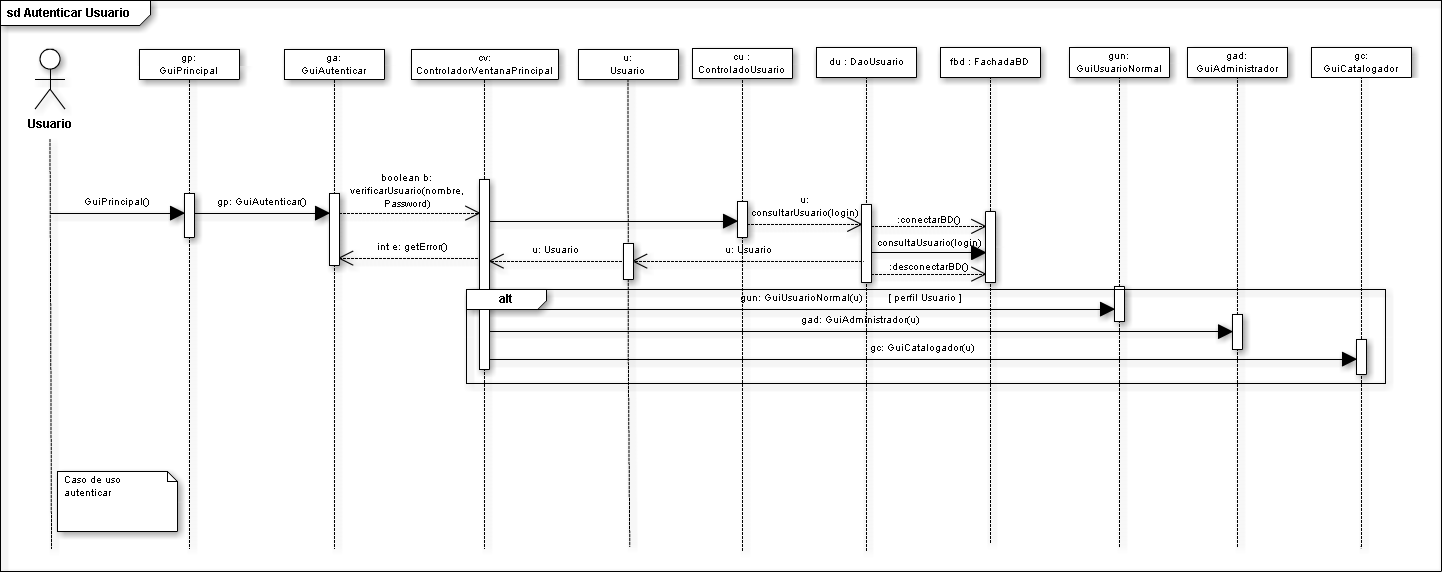
\includegraphics[width=20cm, height=15cm, angle=90]
    			{diagramasSecuencia/AutenticarUsuario}\\[0.5cm]
    			
    			\begin{tabular}{|p{0.225\textwidth}|p{0.225\textwidth}|p{0.225\textwidth}
    			|p{0.225\textwidth}|}
			    \hline
			    {\bf Titulo} & 
			    \multicolumn{3}{p{0.675\textwidth}|}{Diagrama de secuencia Autenticar Usuario}\\
			    \hline
			    \hline
			    {\bf Creador por} & {María Andrea Cruz} & {\bf Fecha} & {Mayo 13 2011}\\
			    \hline
			    \end{tabular}
			    \end{minipage}
			    
			%--------------------------------------------------------------------
			
				\begin{minipage}[c]{1\linewidth}
				\centering
    			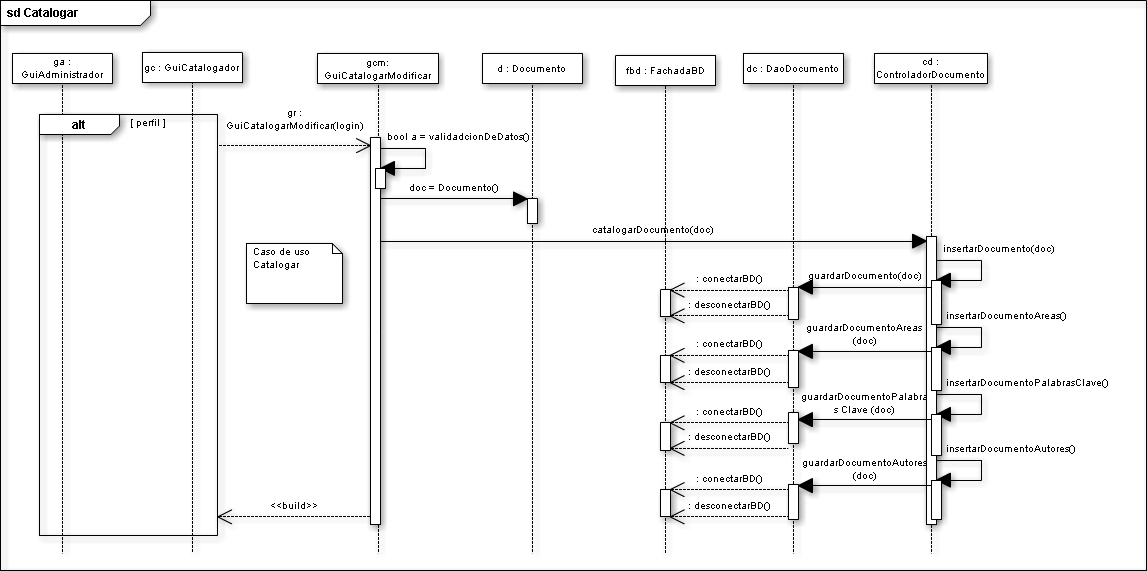
\includegraphics[width=20cm, height=17cm, angle=90]
    			{diagramasSecuencia/Catalogar}\\[0.5cm]
    			
    			\begin{tabular}{|p{0.225\textwidth}|p{0.225\textwidth}|p{0.225\textwidth}
    			|p{0.225\textwidth}|}
			    \hline
			    {\bf Titulo} & 
			    \multicolumn{3}{p{0.675\textwidth}|}{Diagrama de secuencia Catalogar}\\
			    \hline
			    \hline
			    {\bf Creador por} & {Cristian Ríos} & {\bf Fecha} & {Mayo 13 2011}\\
			    \hline
			    \end{tabular}
			    \end{minipage}
			    
			%--------------------------------------------------------------------
			
				\begin{minipage}[c]{1\linewidth}
				\centering
    			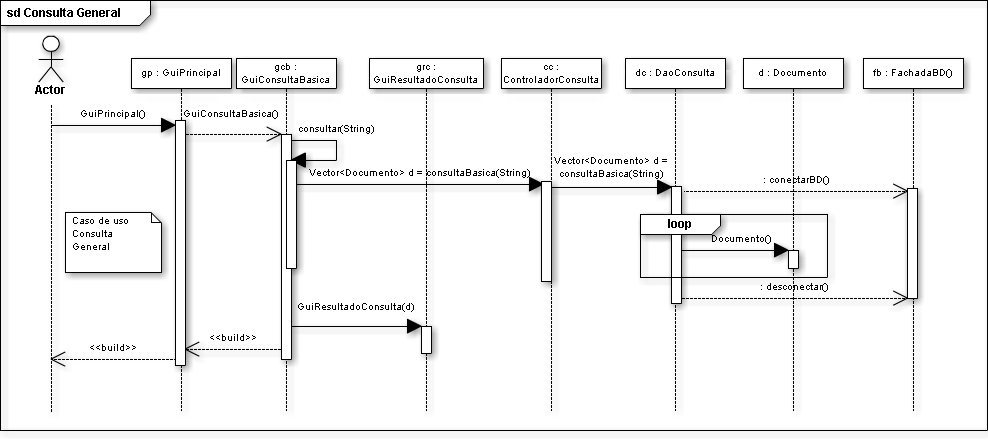
\includegraphics[width=20cm, height=17cm, angle=90]
    			{diagramasSecuencia/ConsultaGeneral}\\[0.5cm]
    			
    			\begin{tabular}{|p{0.225\textwidth}|p{0.225\textwidth}|p{0.225\textwidth}
    			|p{0.225\textwidth}|}
			    \hline
			    {\bf Titulo} & 
			    \multicolumn{3}{p{0.675\textwidth}|}{Diagrama de secuencia Consulta General}\\
			    \hline
			    \hline
			    {\bf Creador por} & {Cristian Ríos} & {\bf Fecha} & {Mayo 14 2011}\\
			    \hline
			    \end{tabular}
			    \end{minipage}
			    
			 %--------------------------------------------------------------------
			
				\begin{minipage}[c]{1\linewidth}
				\centering
    			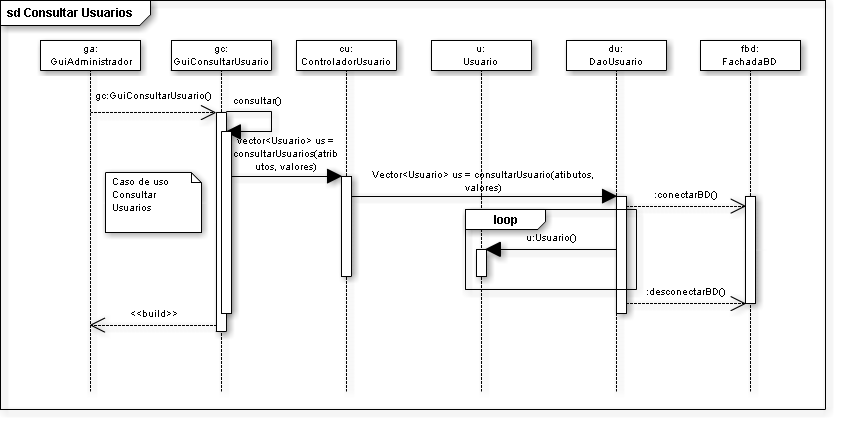
\includegraphics[width=18cm, height=17cm, angle=90]
    			{diagramasSecuencia/ConsultarUsuarios}\\[0.5cm]
    			
    			\begin{tabular}{|p{0.225\textwidth}|p{0.225\textwidth}|p{0.225\textwidth}
    			|p{0.225\textwidth}|}
			    \hline
			    {\bf Titulo} & 
			    \multicolumn{3}{p{0.675\textwidth}|}{Diagrama de secuencia Consultar Usuarios}\\
			    \hline
			    \hline
			    {\bf Creador por} & {Cristian Ríos} & {\bf Fecha} & {Mayo 15 2011}\\
			    \hline
			    \end{tabular}
			    \end{minipage}
			    
			 %--------------------------------------------------------------------
			
				\begin{minipage}[c]{1\linewidth}
				\centering
    			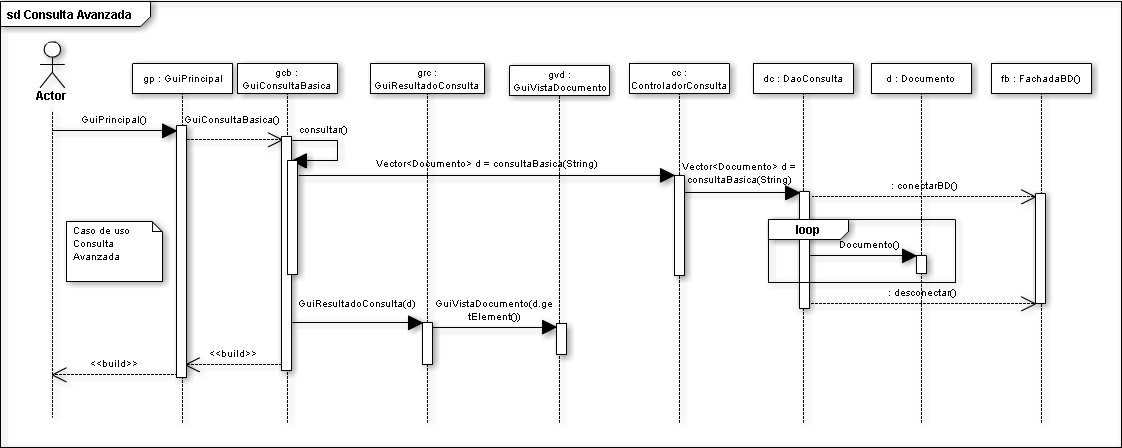
\includegraphics[width=20cm, height=17cm, angle=90]
    			{diagramasSecuencia/ConsultasAvanzadas}\\[0.5cm]
    			
    			\begin{tabular}{|p{0.225\textwidth}|p{0.225\textwidth}|p{0.225\textwidth}
    			|p{0.225\textwidth}|}
			    \hline
			    {\bf Titulo} & 
			    \multicolumn{3}{p{0.675\textwidth}|}{Diagrama de secuencia Consulta Avanzada}\\
			    \hline
			    \hline
			    {\bf Creador por} & {Cristian Ríos} & {\bf Fecha} & {Mayo 14 2011}\\
			    \hline
			    \end{tabular}
			    \end{minipage}
			    
			  %--------------------------------------------------------------------
			
				\begin{minipage}[c]{1\linewidth}
				\centering
    			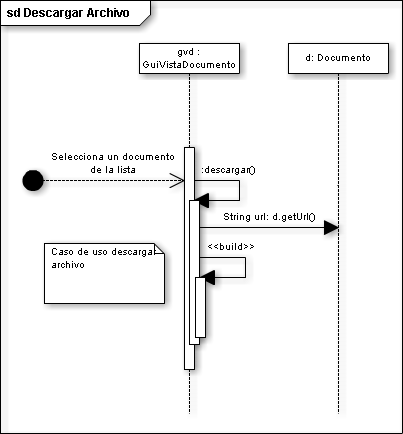
\includegraphics[width=14cm, height=16cm]
    			{diagramasSecuencia/DescargarArchivo}\\[0.5cm]
    			
    			\begin{tabular}{|p{0.225\textwidth}|p{0.225\textwidth}|p{0.225\textwidth}
    			|p{0.225\textwidth}|}
			    \hline
			    {\bf Titulo} & 
			    \multicolumn{3}{p{0.675\textwidth}|}{Diagrama de secuencia Descargar Archivo}\\
			    \hline
			    \hline
			    {\bf Creador por} & {María Andrea Cruz} & {\bf Fecha} & {Mayo 16 2011}\\
			    \hline
			    \end{tabular}
			    \end{minipage}
			    
			 %--------------------------------------------------------------------
			
				\begin{minipage}[c]{1\linewidth}
				\centering
    			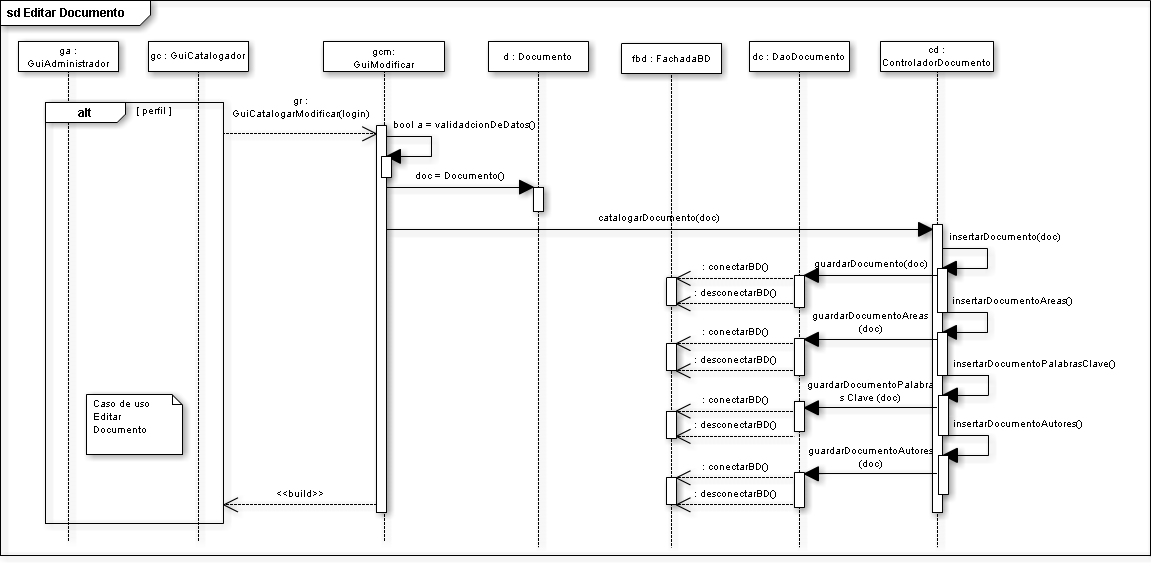
\includegraphics[width=20cm, height=17cm, angle=90]
    			{diagramasSecuencia/EditarDocumento}\\[0.5cm]
    			
    			\begin{tabular}{|p{0.225\textwidth}|p{0.225\textwidth}|p{0.225\textwidth}
    			|p{0.225\textwidth}|}
			    \hline
			    {\bf Titulo} & 
			    \multicolumn{3}{p{0.675\textwidth}|}{Diagrama de secuencia Editar Documento}\\
			    \hline
			    \hline
			    {\bf Creador por} & {Cristian Ríos} & {\bf Fecha} & {Mayo 14 2011}\\
			    \hline
			    \end{tabular}
			    \end{minipage}
			    
			 %--------------------------------------------------------------------
			
				\begin{minipage}[c]{1\linewidth}
				\centering
    			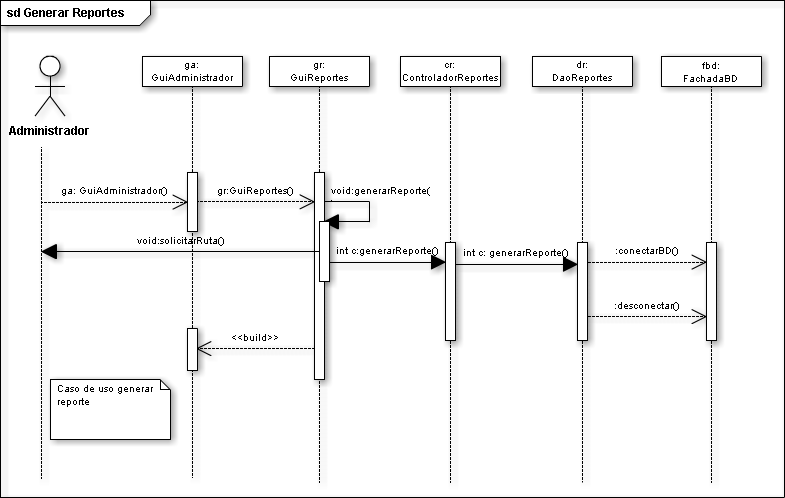
\includegraphics[width=18cm, height=17cm, angle=90]
    			{diagramasSecuencia/GenerarReporte}\\[0.5cm]
    			
    			\begin{tabular}{|p{0.225\textwidth}|p{0.225\textwidth}|p{0.225\textwidth}
    			|p{0.225\textwidth}|}
			    \hline
			    {\bf Titulo} & 
			    \multicolumn{3}{p{0.675\textwidth}|}{Diagrama de secuencia Generar Reportes}\\
			    \hline
			    \hline
			    {\bf Creador por} & {María Andrea Cruz} & {\bf Fecha} & {Mayo 16 2011}\\
			    \hline
			    \end{tabular}
			    \end{minipage}
			    
			 %--------------------------------------------------------------------
			
				\begin{minipage}[c]{1\linewidth}
				\centering
    			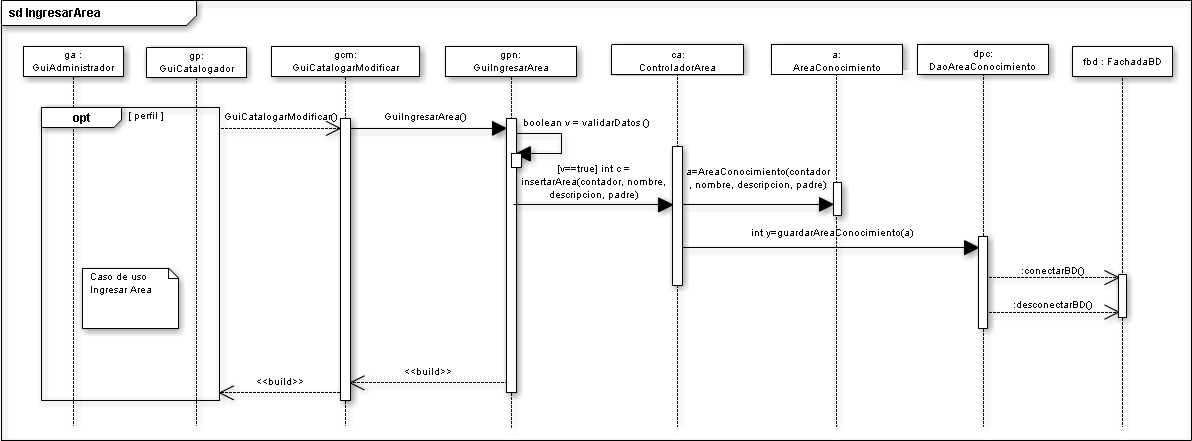
\includegraphics[width=21cm, height=17cm, angle=90]
    			{diagramasSecuencia/IngresarArea}\\[0.5cm]
    			
    			\begin{tabular}{|p{0.225\textwidth}|p{0.225\textwidth}|p{0.225\textwidth}
    			|p{0.225\textwidth}|}
			    \hline
			    {\bf Titulo} & 
			    \multicolumn{3}{p{0.675\textwidth}|}{Diagrama de secuencia Ingresar Área}\\
			    \hline
			    \hline
			    {\bf Creador por} & {Luis Felipe Vargas} & {\bf Fecha} & {Mayo 15 2011}\\
			    \hline
			    \end{tabular}
			    \end{minipage}
			    
			 %--------------------------------------------------------------------
			
				\begin{minipage}[c]{1\linewidth}
				\centering
    			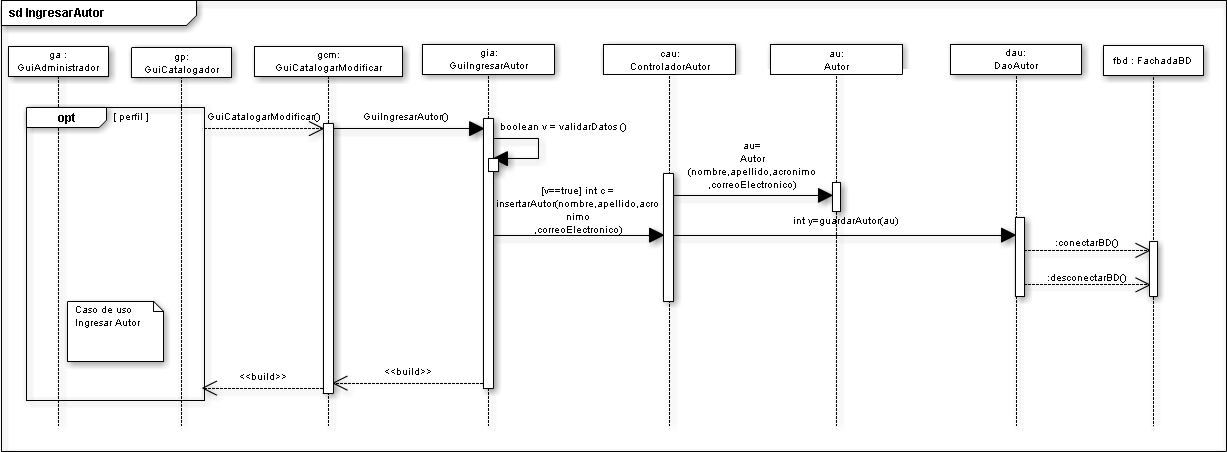
\includegraphics[width=21cm, height=17cm, angle=90]
    			{diagramasSecuencia/IngresarAutor}\\[0.5cm]
    			
    			\begin{tabular}{|p{0.225\textwidth}|p{0.225\textwidth}|p{0.225\textwidth}
    			|p{0.225\textwidth}|}
			    \hline
			    {\bf Titulo} & 
			    \multicolumn{3}{p{0.675\textwidth}|}{Diagrama de secuencia Ingresar Autor}\\
			    \hline
			    \hline
			    {\bf Creador por} & {Luis Felipe Vargas} & {\bf Fecha} & {Mayo 15 2011}\\
			    \hline
			    \end{tabular}
			    \end{minipage}
			    
			 %--------------------------------------------------------------------
			
				\begin{minipage}[c]{1\linewidth}
				\centering
    			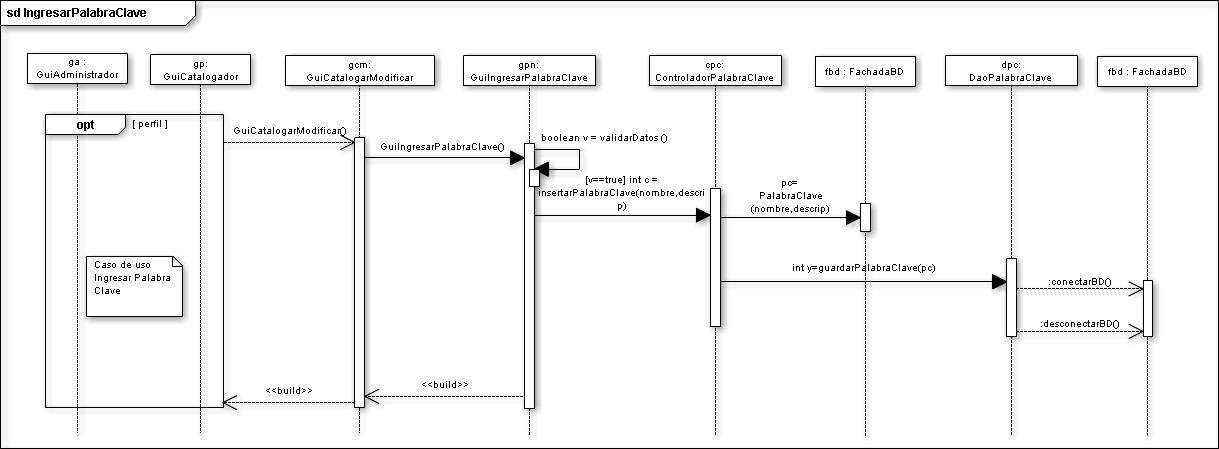
\includegraphics[width=21cm, height=17cm, angle=90]
    			{diagramasSecuencia/IngresarPalabrasClave}\\[0.5cm]
    			
    			\begin{tabular}{|p{0.225\textwidth}|p{0.225\textwidth}|p{0.225\textwidth}
    			|p{0.225\textwidth}|}
			    \hline
			    {\bf Titulo} & 
			    \multicolumn{3}{p{0.675\textwidth}|}{Diagrama de secuencia Ingresar Palabras Claves}\\
			    \hline
			    \hline
			    {\bf Creador por} & {Luis Felipe Vargas} & {\bf Fecha} & {Mayo 15 2011}\\
			    \hline
			    \end{tabular}
			    \end{minipage}
			    
			 %--------------------------------------------------------------------
			
				\begin{minipage}[c]{1\linewidth}
				\centering
    			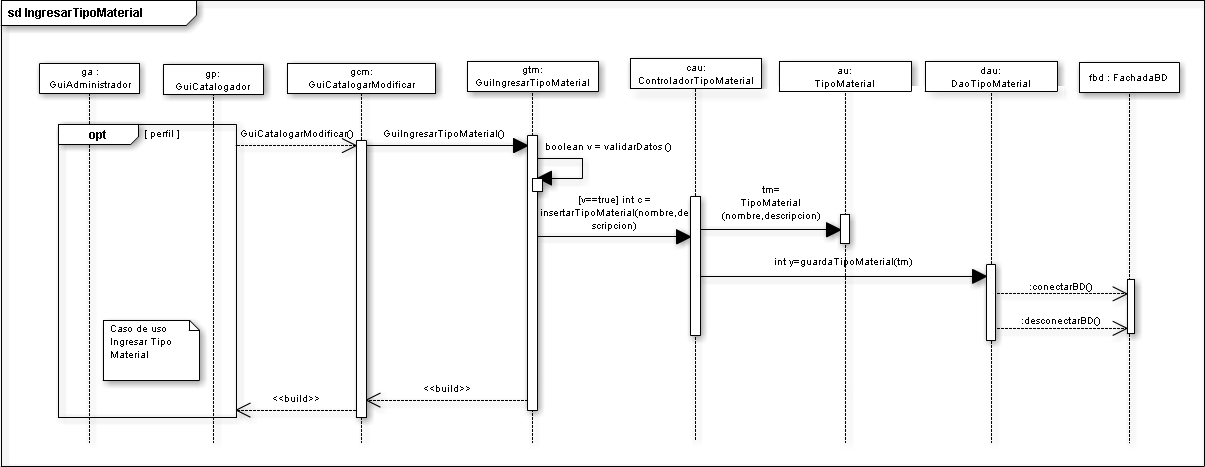
\includegraphics[width=21cm, height=17cm, angle=90]
    			{diagramasSecuencia/IngresarTipoMaterial}\\[0.5cm]
    			
    			\begin{tabular}{|p{0.225\textwidth}|p{0.225\textwidth}|p{0.225\textwidth}
    			|p{0.225\textwidth}|}
			    \hline
			    {\bf Titulo} & 
			    \multicolumn{3}{p{0.675\textwidth}|}{Diagrama de secuencia Ingresar Tipo de Material}\\
			    \hline
			    \hline
			    {\bf Creador por} & {Luis Felipe Vargas} & {\bf Fecha} & {Mayo 15 2011}\\
			    \hline
			    \end{tabular}
			    \end{minipage}
			    
			 %--------------------------------------------------------------------
			
				\begin{minipage}[c]{1\linewidth}
				\centering
    			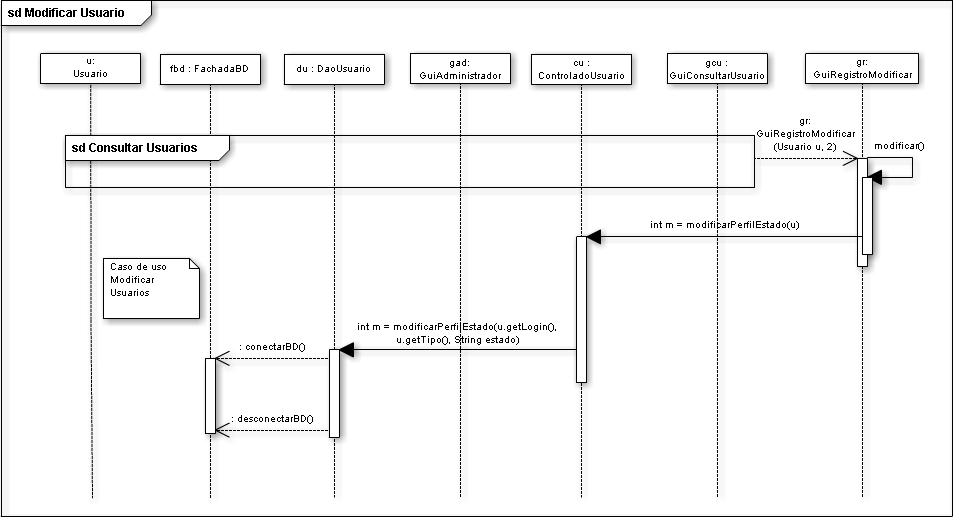
\includegraphics[width=19cm, height=17cm, angle=90]
    			{diagramasSecuencia/ModificarUsuario}\\[0.5cm]
    			
    			\begin{tabular}{|p{0.225\textwidth}|p{0.225\textwidth}|p{0.225\textwidth}
    			|p{0.225\textwidth}|}
			    \hline
			    {\bf Titulo} & 
			    \multicolumn{3}{p{0.675\textwidth}|}{Diagrama de secuencia Modificar Usuarios}\\
			    \hline
			    \hline
			    {\bf Creador por} & {María Andrea Cruz} & {\bf Fecha} & {Mayo 14 2011}\\
			    \hline
			    \end{tabular}
			    \end{minipage}
			    
			 %--------------------------------------------------------------------
			
				\begin{minipage}[c]{1\linewidth}
				\centering
    			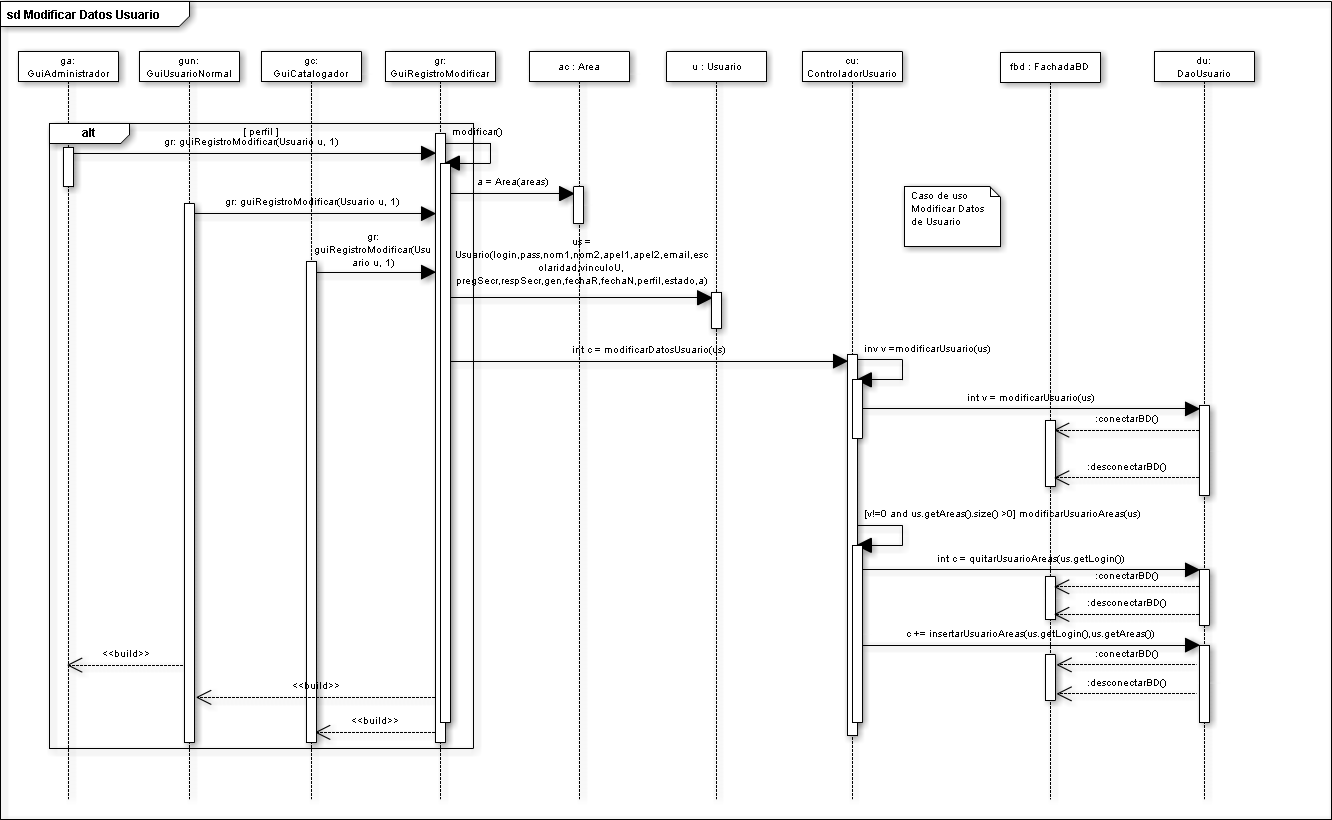
\includegraphics[width=21cm, height=17cm, angle=90]
    			{diagramasSecuencia/ModificarDatos}\\[0.5cm]
    			
    			\begin{tabular}{|p{0.225\textwidth}|p{0.225\textwidth}|p{0.225\textwidth}
    			|p{0.225\textwidth}|}
			    \hline
			    {\bf Titulo} & 
			    \multicolumn{3}{p{0.675\textwidth}|}{Diagrama de secuencia Modificar Datos de Usuario}\\
			    \hline
			    \hline
			    {\bf Creador por} & {Cristian Ríos} & {\bf Fecha} & {Mayo 15 2011}\\
			    \hline
			    \end{tabular}
			    \end{minipage}
			    
			 %--------------------------------------------------------------------
			
				\begin{minipage}[c]{1\linewidth}
				\centering
    			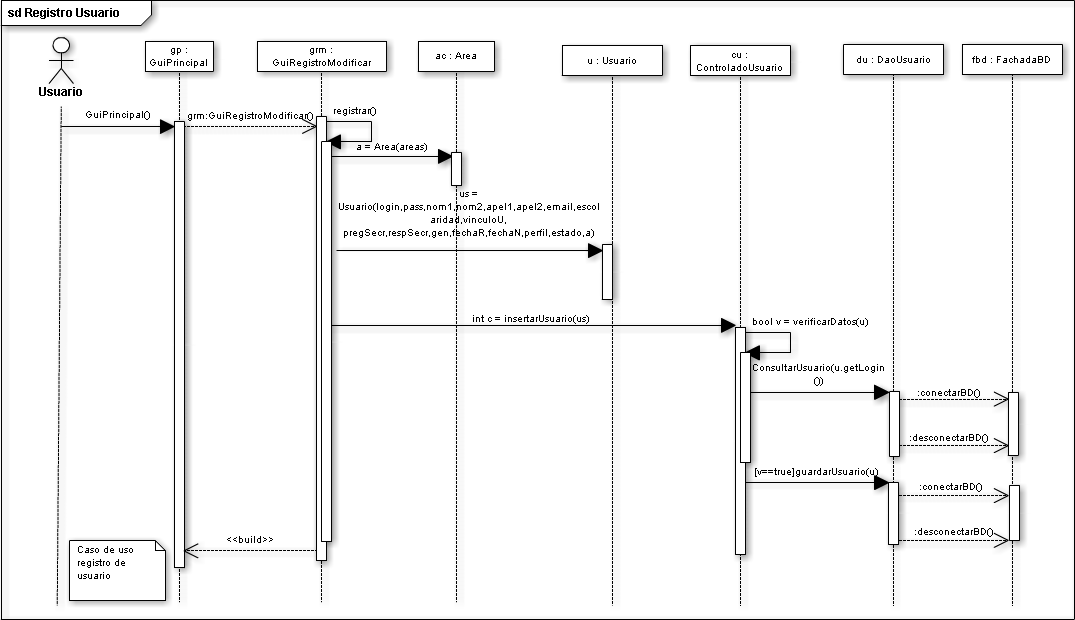
\includegraphics[width=21cm, height=17cm, angle=90]
    			{diagramasSecuencia/RegistroUsuario}\\[0.5cm]
    			
    			\begin{tabular}{|p{0.225\textwidth}|p{0.225\textwidth}|p{0.225\textwidth}
    			|p{0.225\textwidth}|}
			    \hline
			    {\bf Titulo} & 
			    \multicolumn{3}{p{0.675\textwidth}|}{Diagrama de secuencia Registrar Usuario}\\
			    \hline
			    \hline
			    {\bf Creador por} & {Cristian Ríos} & {\bf Fecha} & {Mayo 15 2011}\\
			    \hline
			    \end{tabular}
			    \end{minipage}
			    
			 
			
%\end{document}